\documentclass[11pt]{article}



    \usepackage[T1]{fontenc}
    % Nicer default font (+ math font) than Computer Modern for most use cases
    \usepackage{mathpazo}

    % Basic figure setup, for now with no caption control since it's done
    % automatically by Pandoc (which extracts ![](path) syntax from Markdown).
    \usepackage{graphicx}
    % We will generate all images so they have a width \maxwidth. This means
    % that they will get their normal width if they fit onto the page, but
    % are scaled down if they would overflow the margins.
    \makeatletter
    \def\maxwidth{\ifdim\Gin@nat@width>\linewidth\linewidth
    \else\Gin@nat@width\fi}
    \makeatother
    \let\Oldincludegraphics\includegraphics
    % Set max figure width to be 80% of text width, for now hardcoded.
    \renewcommand{\includegraphics}[1]{\Oldincludegraphics[width=.8\maxwidth]{#1}}
    % Ensure that by default, figures have no caption (until we provide a
    % proper Figure object with a Caption API and a way to capture that
    % in the conversion process - todo).
    \usepackage{caption}
    \DeclareCaptionLabelFormat{nolabel}{}
    \captionsetup{labelformat=nolabel}

    \usepackage{adjustbox} % Used to constrain images to a maximum size
    \usepackage{xcolor} % Allow colors to be defined
    \usepackage{enumerate} % Needed for markdown enumerations to work
    \usepackage{geometry} % Used to adjust the document margins
    \usepackage{amsmath} % Equations
    \usepackage{amssymb} % Equations
    \usepackage{textcomp} % defines textquotesingle
    % Hack from http://tex.stackexchange.com/a/47451/13684:
    \AtBeginDocument{%
        \def\PYZsq{\textquotesingle}% Upright quotes in Pygmentized code
    }
    \usepackage{upquote} % Upright quotes for verbatim code
    \usepackage{eurosym} % defines \euro
    \usepackage[mathletters]{ucs} % Extended unicode (utf-8) support
    \usepackage[utf8x]{inputenc} % Allow utf-8 characters in the tex document
    \usepackage{fancyvrb} % verbatim replacement that allows latex
    \usepackage{grffile} % extends the file name processing of package graphics
                         % to support a larger range
    % The hyperref package gives us a pdf with properly built
    % internal navigation ('pdf bookmarks' for the table of contents,
    % internal cross-reference links, web links for URLs, etc.)
    \usepackage{hyperref}
    \usepackage{longtable} % longtable support required by pandoc >1.10
    \usepackage{booktabs}  % table support for pandoc > 1.12.2
    \usepackage[inline]{enumitem} % IRkernel/repr support (it uses the enumerate* environment)
    \usepackage[normalem]{ulem} % ulem is needed to support strikethroughs (\sout)
                                % normalem makes italics be italics, not underlines


                                    % novos pacotes
                                    \usepackage[font=scriptsize]{caption}
                                    \usepackage{float}


    % Colors for the hyperref package
    \definecolor{urlcolor}{rgb}{0,.145,.698}
    \definecolor{linkcolor}{rgb}{.71,0.21,0.01}
    \definecolor{citecolor}{rgb}{.12,.54,.11}

    % ANSI colors
    \definecolor{ansi-black}{HTML}{3E424D}
    \definecolor{ansi-black-intense}{HTML}{282C36}
    \definecolor{ansi-red}{HTML}{E75C58}
    \definecolor{ansi-red-intense}{HTML}{B22B31}
    \definecolor{ansi-green}{HTML}{00A250}
    \definecolor{ansi-green-intense}{HTML}{007427}
    \definecolor{ansi-yellow}{HTML}{DDB62B}
    \definecolor{ansi-yellow-intense}{HTML}{B27D12}
    \definecolor{ansi-blue}{HTML}{208FFB}
    \definecolor{ansi-blue-intense}{HTML}{0065CA}
    \definecolor{ansi-magenta}{HTML}{D160C4}
    \definecolor{ansi-magenta-intense}{HTML}{A03196}
    \definecolor{ansi-cyan}{HTML}{60C6C8}
    \definecolor{ansi-cyan-intense}{HTML}{258F8F}
    \definecolor{ansi-white}{HTML}{C5C1B4}
    \definecolor{ansi-white-intense}{HTML}{A1A6B2}

    % commands and environments needed by pandoc snippets
    % extracted from the output of `pandoc -s`
    \providecommand{\tightlist}{%
      \setlength{\itemsep}{0pt}\setlength{\parskip}{0pt}}
    \DefineVerbatimEnvironment{Highlighting}{Verbatim}{commandchars=\\\{\}}
    % Add ',fontsize=\small' for more characters per line
    \newenvironment{Shaded}{}{}
    \newcommand{\KeywordTok}[1]{\textcolor[rgb]{0.00,0.44,0.13}{\textbf{{#1}}}}
    \newcommand{\DataTypeTok}[1]{\textcolor[rgb]{0.56,0.13,0.00}{{#1}}}
    \newcommand{\DecValTok}[1]{\textcolor[rgb]{0.25,0.63,0.44}{{#1}}}
    \newcommand{\BaseNTok}[1]{\textcolor[rgb]{0.25,0.63,0.44}{{#1}}}
    \newcommand{\FloatTok}[1]{\textcolor[rgb]{0.25,0.63,0.44}{{#1}}}
    \newcommand{\CharTok}[1]{\textcolor[rgb]{0.25,0.44,0.63}{{#1}}}
    \newcommand{\StringTok}[1]{\textcolor[rgb]{0.25,0.44,0.63}{{#1}}}
    \newcommand{\CommentTok}[1]{\textcolor[rgb]{0.38,0.63,0.69}{\textit{{#1}}}}
    \newcommand{\OtherTok}[1]{\textcolor[rgb]{0.00,0.44,0.13}{{#1}}}
    \newcommand{\AlertTok}[1]{\textcolor[rgb]{1.00,0.00,0.00}{\textbf{{#1}}}}
    \newcommand{\FunctionTok}[1]{\textcolor[rgb]{0.02,0.16,0.49}{{#1}}}
    \newcommand{\RegionMarkerTok}[1]{{#1}}
    \newcommand{\ErrorTok}[1]{\textcolor[rgb]{1.00,0.00,0.00}{\textbf{{#1}}}}
    \newcommand{\NormalTok}[1]{{#1}}

    % Additional commands for more recent versions of Pandoc
    \newcommand{\ConstantTok}[1]{\textcolor[rgb]{0.53,0.00,0.00}{{#1}}}
    \newcommand{\SpecialCharTok}[1]{\textcolor[rgb]{0.25,0.44,0.63}{{#1}}}
    \newcommand{\VerbatimStringTok}[1]{\textcolor[rgb]{0.25,0.44,0.63}{{#1}}}
    \newcommand{\SpecialStringTok}[1]{\textcolor[rgb]{0.73,0.40,0.53}{{#1}}}
    \newcommand{\ImportTok}[1]{{#1}}
    \newcommand{\DocumentationTok}[1]{\textcolor[rgb]{0.73,0.13,0.13}{\textit{{#1}}}}
    \newcommand{\AnnotationTok}[1]{\textcolor[rgb]{0.38,0.63,0.69}{\textbf{\textit{{#1}}}}}
    \newcommand{\CommentVarTok}[1]{\textcolor[rgb]{0.38,0.63,0.69}{\textbf{\textit{{#1}}}}}
    \newcommand{\VariableTok}[1]{\textcolor[rgb]{0.10,0.09,0.49}{{#1}}}
    \newcommand{\ControlFlowTok}[1]{\textcolor[rgb]{0.00,0.44,0.13}{\textbf{{#1}}}}
    \newcommand{\OperatorTok}[1]{\textcolor[rgb]{0.40,0.40,0.40}{{#1}}}
    \newcommand{\BuiltInTok}[1]{{#1}}
    \newcommand{\ExtensionTok}[1]{{#1}}
    \newcommand{\PreprocessorTok}[1]{\textcolor[rgb]{0.74,0.48,0.00}{{#1}}}
    \newcommand{\AttributeTok}[1]{\textcolor[rgb]{0.49,0.56,0.16}{{#1}}}
    \newcommand{\InformationTok}[1]{\textcolor[rgb]{0.38,0.63,0.69}{\textbf{\textit{{#1}}}}}
    \newcommand{\WarningTok}[1]{\textcolor[rgb]{0.38,0.63,0.69}{\textbf{\textit{{#1}}}}}


    % Define a nice break command that doesn't care if a line doesn't already
    % exist.
    \def\br{\hspace*{\fill} \\* }
    % Math Jax compatability definitions
    \def\gt{>}
    \def\lt{<}
    % Document parameters
    \title{lista03\_resolucao}




    % Pygments definitions

\makeatletter
\def\PY@reset{\let\PY@it=\relax \let\PY@bf=\relax%
    \let\PY@ul=\relax \let\PY@tc=\relax%
    \let\PY@bc=\relax \let\PY@ff=\relax}
\def\PY@tok#1{\csname PY@tok@#1\endcsname}
\def\PY@toks#1+{\ifx\relax#1\empty\else%
    \PY@tok{#1}\expandafter\PY@toks\fi}
\def\PY@do#1{\PY@bc{\PY@tc{\PY@ul{%
    \PY@it{\PY@bf{\PY@ff{#1}}}}}}}
\def\PY#1#2{\PY@reset\PY@toks#1+\relax+\PY@do{#2}}

\expandafter\def\csname PY@tok@gd\endcsname{\def\PY@tc##1{\textcolor[rgb]{0.63,0.00,0.00}{##1}}}
\expandafter\def\csname PY@tok@gu\endcsname{\let\PY@bf=\textbf\def\PY@tc##1{\textcolor[rgb]{0.50,0.00,0.50}{##1}}}
\expandafter\def\csname PY@tok@gt\endcsname{\def\PY@tc##1{\textcolor[rgb]{0.00,0.27,0.87}{##1}}}
\expandafter\def\csname PY@tok@gs\endcsname{\let\PY@bf=\textbf}
\expandafter\def\csname PY@tok@gr\endcsname{\def\PY@tc##1{\textcolor[rgb]{1.00,0.00,0.00}{##1}}}
\expandafter\def\csname PY@tok@cm\endcsname{\let\PY@it=\textit\def\PY@tc##1{\textcolor[rgb]{0.25,0.50,0.50}{##1}}}
\expandafter\def\csname PY@tok@vg\endcsname{\def\PY@tc##1{\textcolor[rgb]{0.10,0.09,0.49}{##1}}}
\expandafter\def\csname PY@tok@vi\endcsname{\def\PY@tc##1{\textcolor[rgb]{0.10,0.09,0.49}{##1}}}
\expandafter\def\csname PY@tok@mh\endcsname{\def\PY@tc##1{\textcolor[rgb]{0.40,0.40,0.40}{##1}}}
\expandafter\def\csname PY@tok@cs\endcsname{\let\PY@it=\textit\def\PY@tc##1{\textcolor[rgb]{0.25,0.50,0.50}{##1}}}
\expandafter\def\csname PY@tok@ge\endcsname{\let\PY@it=\textit}
\expandafter\def\csname PY@tok@vc\endcsname{\def\PY@tc##1{\textcolor[rgb]{0.10,0.09,0.49}{##1}}}
\expandafter\def\csname PY@tok@il\endcsname{\def\PY@tc##1{\textcolor[rgb]{0.40,0.40,0.40}{##1}}}
\expandafter\def\csname PY@tok@go\endcsname{\def\PY@tc##1{\textcolor[rgb]{0.53,0.53,0.53}{##1}}}
\expandafter\def\csname PY@tok@cp\endcsname{\def\PY@tc##1{\textcolor[rgb]{0.74,0.48,0.00}{##1}}}
\expandafter\def\csname PY@tok@gi\endcsname{\def\PY@tc##1{\textcolor[rgb]{0.00,0.63,0.00}{##1}}}
\expandafter\def\csname PY@tok@gh\endcsname{\let\PY@bf=\textbf\def\PY@tc##1{\textcolor[rgb]{0.00,0.00,0.50}{##1}}}
\expandafter\def\csname PY@tok@ni\endcsname{\let\PY@bf=\textbf\def\PY@tc##1{\textcolor[rgb]{0.60,0.60,0.60}{##1}}}
\expandafter\def\csname PY@tok@nl\endcsname{\def\PY@tc##1{\textcolor[rgb]{0.63,0.63,0.00}{##1}}}
\expandafter\def\csname PY@tok@nn\endcsname{\let\PY@bf=\textbf\def\PY@tc##1{\textcolor[rgb]{0.00,0.00,1.00}{##1}}}
\expandafter\def\csname PY@tok@no\endcsname{\def\PY@tc##1{\textcolor[rgb]{0.53,0.00,0.00}{##1}}}
\expandafter\def\csname PY@tok@na\endcsname{\def\PY@tc##1{\textcolor[rgb]{0.49,0.56,0.16}{##1}}}
\expandafter\def\csname PY@tok@nb\endcsname{\def\PY@tc##1{\textcolor[rgb]{0.00,0.50,0.00}{##1}}}
\expandafter\def\csname PY@tok@nc\endcsname{\let\PY@bf=\textbf\def\PY@tc##1{\textcolor[rgb]{0.00,0.00,1.00}{##1}}}
\expandafter\def\csname PY@tok@nd\endcsname{\def\PY@tc##1{\textcolor[rgb]{0.67,0.13,1.00}{##1}}}
\expandafter\def\csname PY@tok@ne\endcsname{\let\PY@bf=\textbf\def\PY@tc##1{\textcolor[rgb]{0.82,0.25,0.23}{##1}}}
\expandafter\def\csname PY@tok@nf\endcsname{\def\PY@tc##1{\textcolor[rgb]{0.00,0.00,1.00}{##1}}}
\expandafter\def\csname PY@tok@si\endcsname{\let\PY@bf=\textbf\def\PY@tc##1{\textcolor[rgb]{0.73,0.40,0.53}{##1}}}
\expandafter\def\csname PY@tok@s2\endcsname{\def\PY@tc##1{\textcolor[rgb]{0.73,0.13,0.13}{##1}}}
\expandafter\def\csname PY@tok@nt\endcsname{\let\PY@bf=\textbf\def\PY@tc##1{\textcolor[rgb]{0.00,0.50,0.00}{##1}}}
\expandafter\def\csname PY@tok@nv\endcsname{\def\PY@tc##1{\textcolor[rgb]{0.10,0.09,0.49}{##1}}}
\expandafter\def\csname PY@tok@s1\endcsname{\def\PY@tc##1{\textcolor[rgb]{0.73,0.13,0.13}{##1}}}
\expandafter\def\csname PY@tok@ch\endcsname{\let\PY@it=\textit\def\PY@tc##1{\textcolor[rgb]{0.25,0.50,0.50}{##1}}}
\expandafter\def\csname PY@tok@m\endcsname{\def\PY@tc##1{\textcolor[rgb]{0.40,0.40,0.40}{##1}}}
\expandafter\def\csname PY@tok@gp\endcsname{\let\PY@bf=\textbf\def\PY@tc##1{\textcolor[rgb]{0.00,0.00,0.50}{##1}}}
\expandafter\def\csname PY@tok@sh\endcsname{\def\PY@tc##1{\textcolor[rgb]{0.73,0.13,0.13}{##1}}}
\expandafter\def\csname PY@tok@ow\endcsname{\let\PY@bf=\textbf\def\PY@tc##1{\textcolor[rgb]{0.67,0.13,1.00}{##1}}}
\expandafter\def\csname PY@tok@sx\endcsname{\def\PY@tc##1{\textcolor[rgb]{0.00,0.50,0.00}{##1}}}
\expandafter\def\csname PY@tok@bp\endcsname{\def\PY@tc##1{\textcolor[rgb]{0.00,0.50,0.00}{##1}}}
\expandafter\def\csname PY@tok@c1\endcsname{\let\PY@it=\textit\def\PY@tc##1{\textcolor[rgb]{0.25,0.50,0.50}{##1}}}
\expandafter\def\csname PY@tok@o\endcsname{\def\PY@tc##1{\textcolor[rgb]{0.40,0.40,0.40}{##1}}}
\expandafter\def\csname PY@tok@kc\endcsname{\let\PY@bf=\textbf\def\PY@tc##1{\textcolor[rgb]{0.00,0.50,0.00}{##1}}}
\expandafter\def\csname PY@tok@c\endcsname{\let\PY@it=\textit\def\PY@tc##1{\textcolor[rgb]{0.25,0.50,0.50}{##1}}}
\expandafter\def\csname PY@tok@mf\endcsname{\def\PY@tc##1{\textcolor[rgb]{0.40,0.40,0.40}{##1}}}
\expandafter\def\csname PY@tok@err\endcsname{\def\PY@bc##1{\setlength{\fboxsep}{0pt}\fcolorbox[rgb]{1.00,0.00,0.00}{1,1,1}{\strut ##1}}}
\expandafter\def\csname PY@tok@mb\endcsname{\def\PY@tc##1{\textcolor[rgb]{0.40,0.40,0.40}{##1}}}
\expandafter\def\csname PY@tok@ss\endcsname{\def\PY@tc##1{\textcolor[rgb]{0.10,0.09,0.49}{##1}}}
\expandafter\def\csname PY@tok@sr\endcsname{\def\PY@tc##1{\textcolor[rgb]{0.73,0.40,0.53}{##1}}}
\expandafter\def\csname PY@tok@mo\endcsname{\def\PY@tc##1{\textcolor[rgb]{0.40,0.40,0.40}{##1}}}
\expandafter\def\csname PY@tok@kd\endcsname{\let\PY@bf=\textbf\def\PY@tc##1{\textcolor[rgb]{0.00,0.50,0.00}{##1}}}
\expandafter\def\csname PY@tok@mi\endcsname{\def\PY@tc##1{\textcolor[rgb]{0.40,0.40,0.40}{##1}}}
\expandafter\def\csname PY@tok@kn\endcsname{\let\PY@bf=\textbf\def\PY@tc##1{\textcolor[rgb]{0.00,0.50,0.00}{##1}}}
\expandafter\def\csname PY@tok@cpf\endcsname{\let\PY@it=\textit\def\PY@tc##1{\textcolor[rgb]{0.25,0.50,0.50}{##1}}}
\expandafter\def\csname PY@tok@kr\endcsname{\let\PY@bf=\textbf\def\PY@tc##1{\textcolor[rgb]{0.00,0.50,0.00}{##1}}}
\expandafter\def\csname PY@tok@s\endcsname{\def\PY@tc##1{\textcolor[rgb]{0.73,0.13,0.13}{##1}}}
\expandafter\def\csname PY@tok@kp\endcsname{\def\PY@tc##1{\textcolor[rgb]{0.00,0.50,0.00}{##1}}}
\expandafter\def\csname PY@tok@w\endcsname{\def\PY@tc##1{\textcolor[rgb]{0.73,0.73,0.73}{##1}}}
\expandafter\def\csname PY@tok@kt\endcsname{\def\PY@tc##1{\textcolor[rgb]{0.69,0.00,0.25}{##1}}}
\expandafter\def\csname PY@tok@sc\endcsname{\def\PY@tc##1{\textcolor[rgb]{0.73,0.13,0.13}{##1}}}
\expandafter\def\csname PY@tok@sb\endcsname{\def\PY@tc##1{\textcolor[rgb]{0.73,0.13,0.13}{##1}}}
\expandafter\def\csname PY@tok@k\endcsname{\let\PY@bf=\textbf\def\PY@tc##1{\textcolor[rgb]{0.00,0.50,0.00}{##1}}}
\expandafter\def\csname PY@tok@se\endcsname{\let\PY@bf=\textbf\def\PY@tc##1{\textcolor[rgb]{0.73,0.40,0.13}{##1}}}
\expandafter\def\csname PY@tok@sd\endcsname{\let\PY@it=\textit\def\PY@tc##1{\textcolor[rgb]{0.73,0.13,0.13}{##1}}}

\def\PYZbs{\char`\\}
\def\PYZus{\char`\_}
\def\PYZob{\char`\{}
\def\PYZcb{\char`\}}
\def\PYZca{\char`\^}
\def\PYZam{\char`\&}
\def\PYZlt{\char`\<}
\def\PYZgt{\char`\>}
\def\PYZsh{\char`\#}
\def\PYZpc{\char`\%}
\def\PYZdl{\char`\$}
\def\PYZhy{\char`\-}
\def\PYZsq{\char`\'}
\def\PYZdq{\char`\"}
\def\PYZti{\char`\~}
% for compatibility with earlier versions
\def\PYZat{@}
\def\PYZlb{[}
\def\PYZrb{]}
\makeatother


    % Exact colors from NB
    \definecolor{incolor}{rgb}{0.0, 0.0, 0.5}
    \definecolor{outcolor}{rgb}{0.545, 0.0, 0.0}




    % Prevent overflowing lines due to hard-to-break entities
    \sloppy
    % Setup hyperref package
    \hypersetup{
      breaklinks=true,  % so long urls are correctly broken across lines
      colorlinks=true,
      urlcolor=urlcolor,
      linkcolor=linkcolor,
      citecolor=citecolor,
      }
    % Slightly bigger margins than the latex defaults

    \geometry{verbose,tmargin=1in,bmargin=1in,lmargin=1in,rmargin=1in}



    \begin{document}

\title{Lista 1 - IOF814: Modelos Numéricos Aplicados a Processos Costeiros e Estuarinos}
\maketitle

\begin{center}
\textbf{Aluno:} Danilo Augusto Silva

\textbf{Nº USP:} 7279456

\textbf{Data de Entrega:} 31 de Outubro/2017
\end{center}
\vspace{0.5in}
Informações gerais quanto a estrutura da lista:

codes/: contem os códigos elaborados para os exercícios;

data/: contem os arquivos de input para alguns códigos e

outputs/: contem os arquivos de saída dos códigos, armazenados em
subpastas designada para cada questão, bem como o arquivo original \textbf{.tex}
e \textbf{.pdf} desta lista, com os desenvolvimentos das discretizações e
respostas dissertativas.

    \subparagraph{Exercício 1}\label{exercuxedcio-1}

Baseado em uma condição inicial de repouso, a influência do vento em
toda a coluna de água só foi observado a partir de 30 minutos de
simulação. Desta forma, as imagens apresentadas são do último instante
de tempo simulado, após um tempo de aquecimento do modelo para
estabilidade do mesmo.

A principal diferença entre as simulações realizadas para cada latitude,
se dá a partir de 30m de profundidade, onde a orientação dos vetores
sofre uma deflecção maior conforme a latitude aumenta. Para \(30^oS\) os
vetores a 30m são quase zonais, com um pequeno ângulo de deflecção para
a esquerda do sentido da corrente (Fig 1.1). Já para os ângulos
\(45^oS\) e \(60^oS\), essa deflecção aumenta, rumando para uma
orientação para noroeste (Fig 1.2 e 1.3).

Essa variação na deflecção também é observada em camadas mais rasas,
onde os vetores sofrem uma deflecção sentido horário, passando de
sudoeste (Fig. 1.1)para oeste (Fig 1.3).

Desta forma, concluímos que o aumento da latitude influenciará a
resposta do oceano a um vento homogêneo e uniforme, no sentido de
defletir as correntes geradas no sentido horário da propagação do vento.

\begin{figure}[!ht]
\centering
\centerline{\hbox{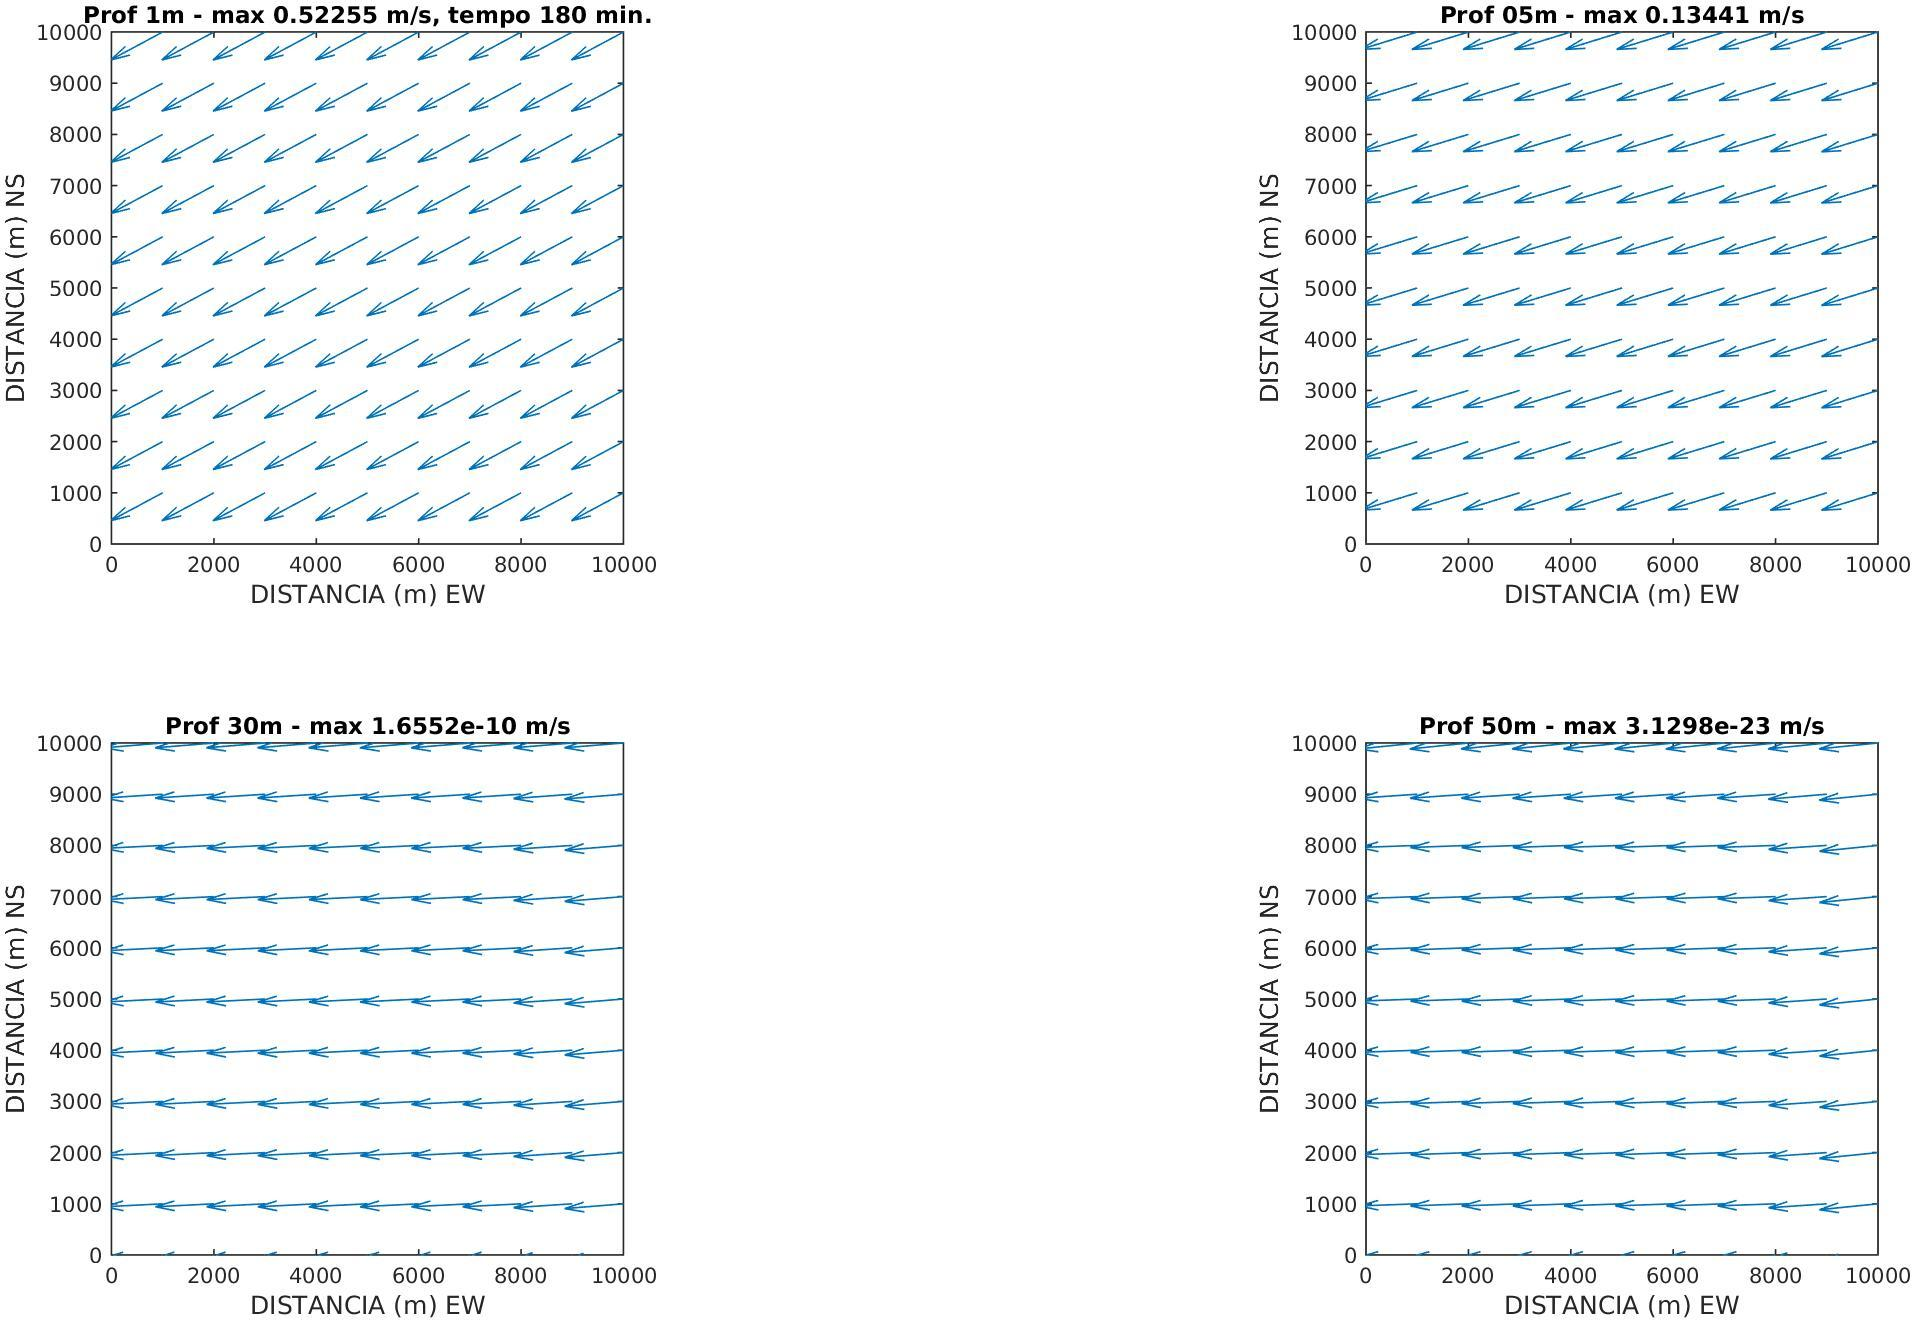
\includegraphics{/home/tparente/danilo/mestrado/github/IOF814/Lista03/outputs/ex01/vento30_360.png}}}
\caption{Fig 1.1 - reposta do oceano a um vento homogêneo de NE nas profundidades de 1m, 5m, 30m e 50m.}
\label{fig1:1}
\end{figure}

\begin{figure}[!ht]
\centering
\centerline{\hbox{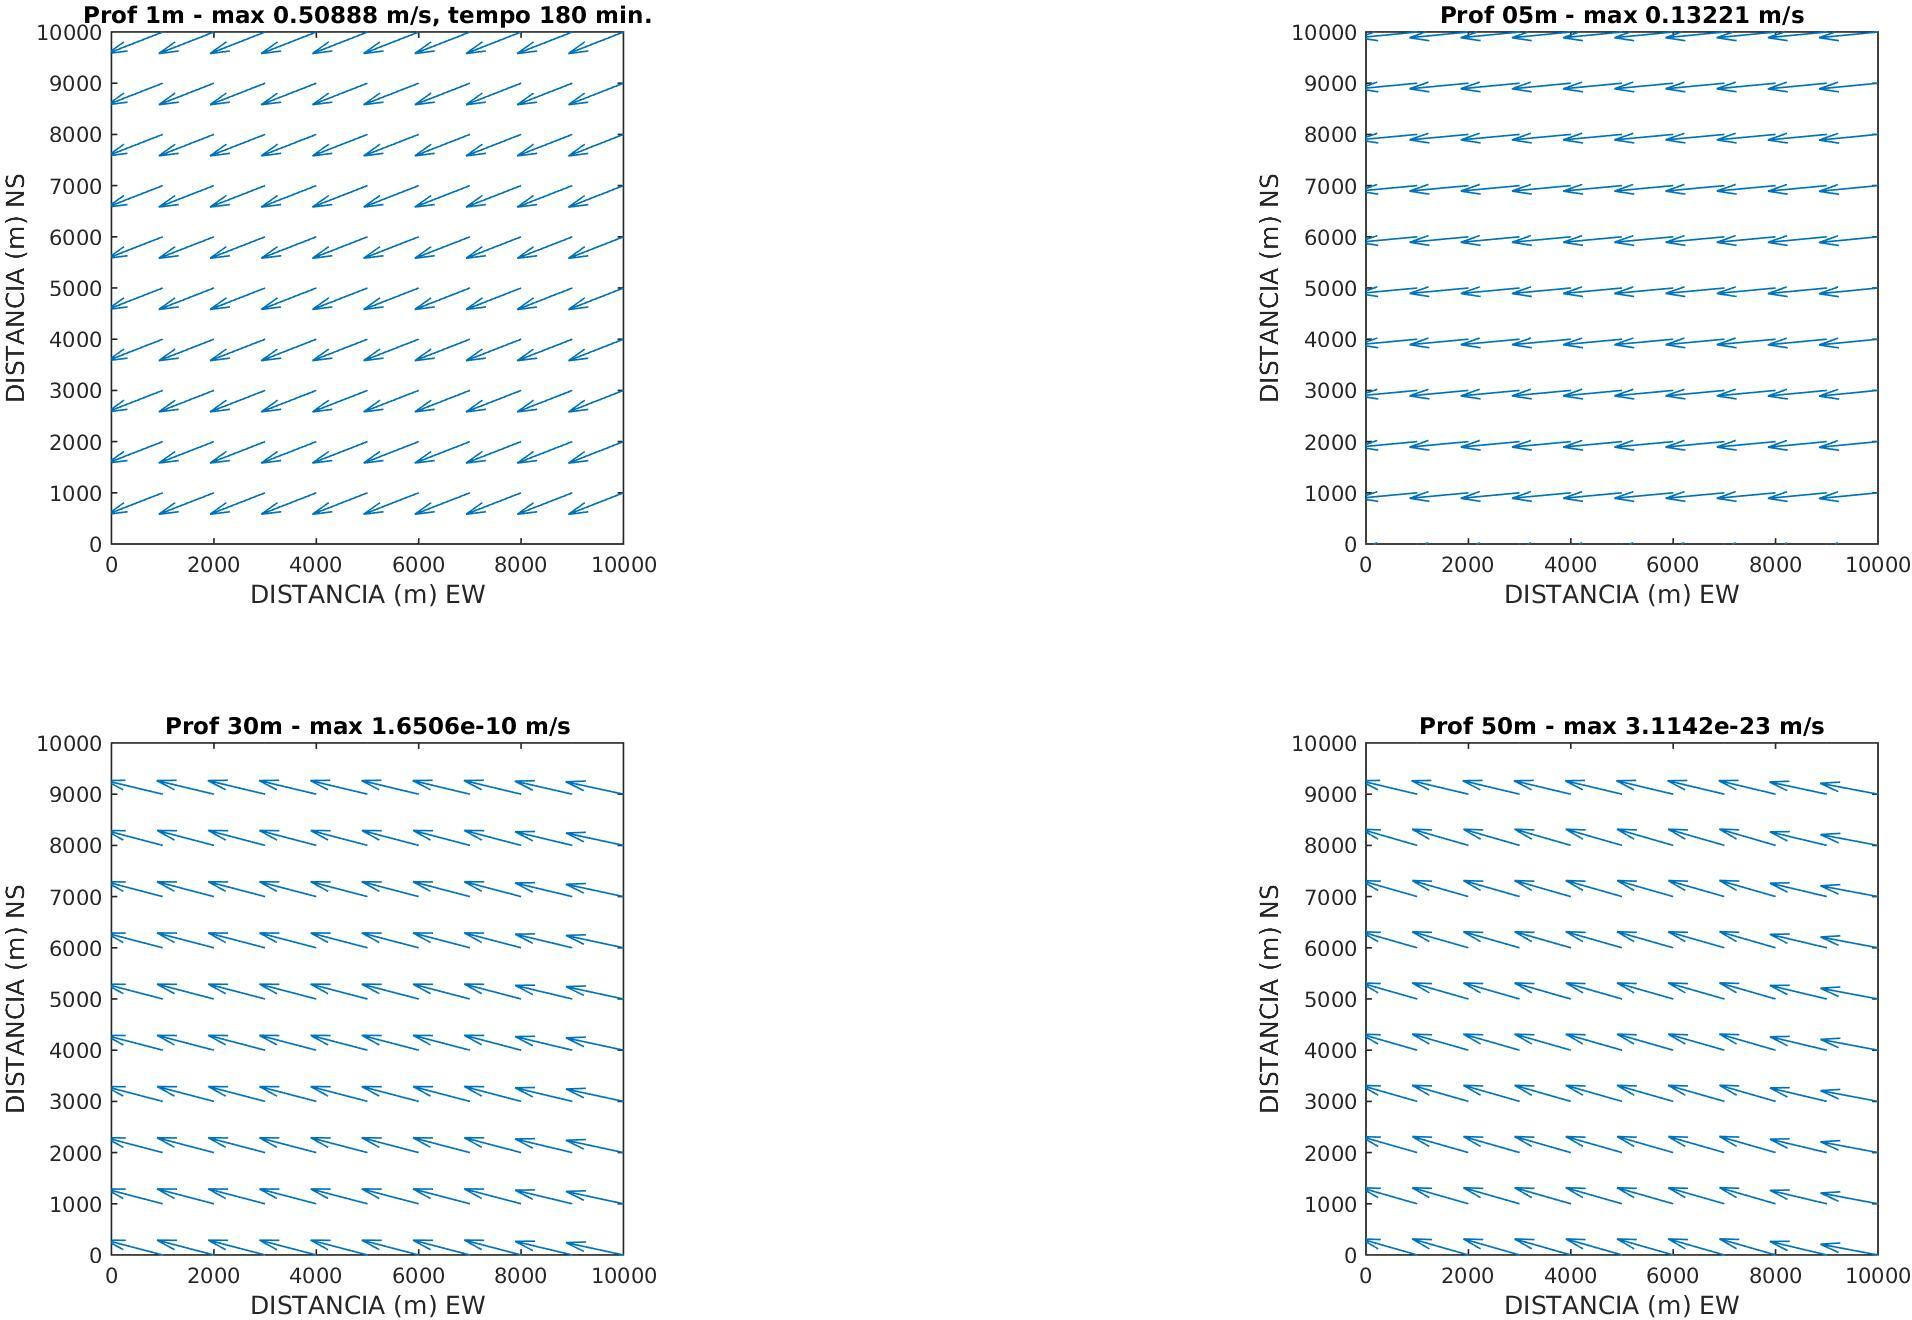
\includegraphics{/home/tparente/danilo/mestrado/github/IOF814/Lista03/outputs/ex01/vento45_360.png}}}
\caption{Fig 1.2 - reposta do oceano a um vento homogêneo de NE nas profundidades de 1m, 5m, 30m e 50m.}
\label{fig1:2}
\end{figure}

\begin{figure}[!ht]
\centering
\centerline{\hbox{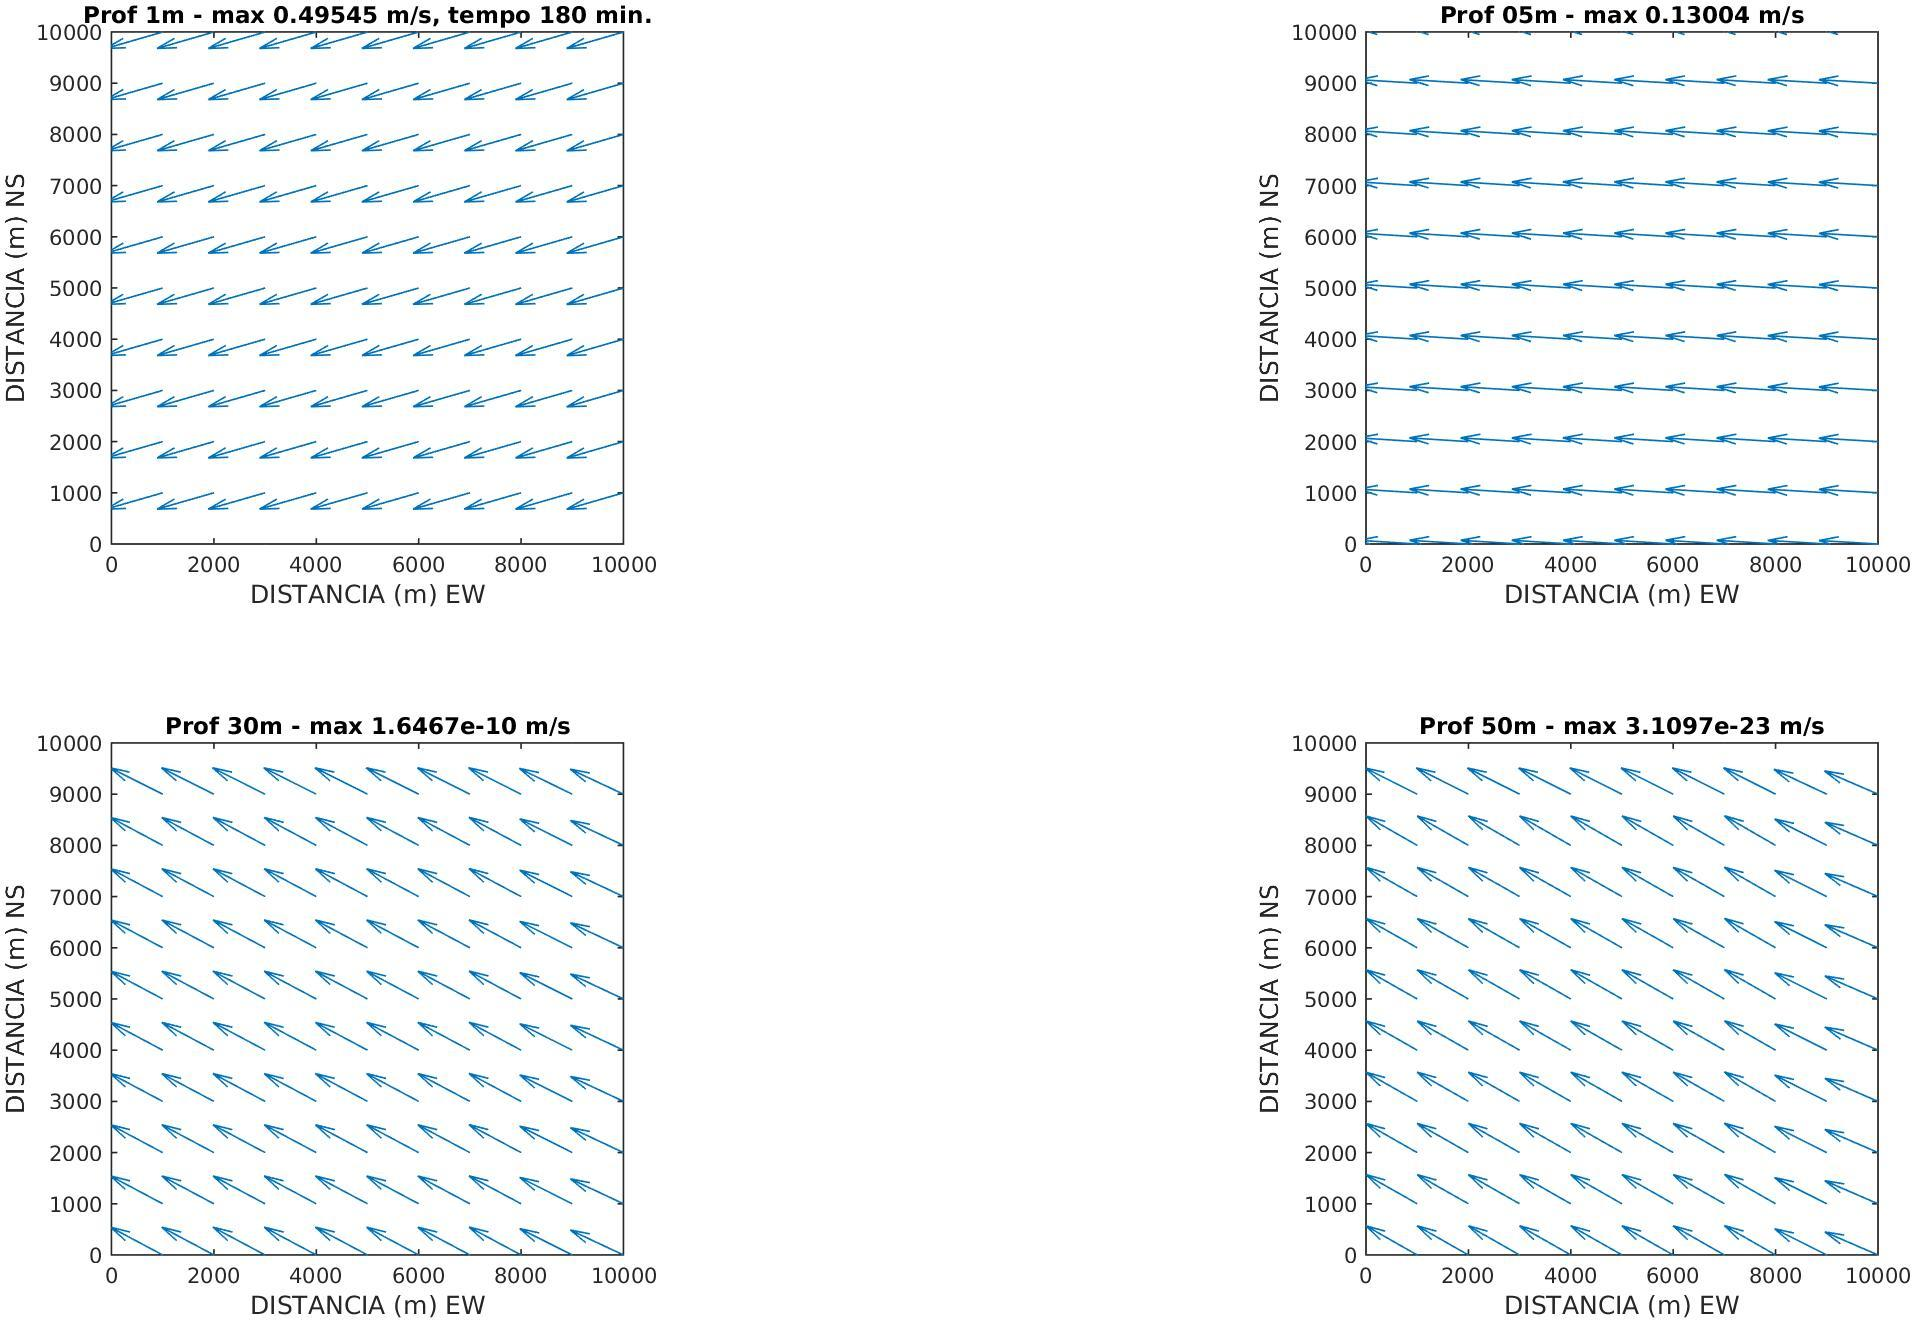
\includegraphics{/home/tparente/danilo/mestrado/github/IOF814/Lista03/outputs/ex01/vento60_360.png}}}
\caption{Fig 1.3 - reposta do oceano a um vento homogêneo de NE nas profundidades de 1m, 5m, 30m e 50m.}
\label{fig1:3}
\end{figure}

\newpage
    \subparagraph{Exercício 2}\label{exercuxedcio-2}

Um modelo de duas camadas consiste em um modelo teórico, onde o oceano
pode ser aproximado para duas camadas de densidades diferentes e
constantes em cada camada (Figura 2.1).

Sendo assim, não há cálculos de corrente vertical, como em um modelo 3D,
onde somente são apresentadas as médias da velocidade vertical em cada
camada.

As tensões envolvidas nas camadas estão relacionadas a fricção entre
camadas, na interface entre elas. No limite superior da camada superior,
a tensão de cisalhamento do vento é uma das principais forçantes em
inserir energia no sistema oceânico, gerando movimento, enquanto que no
limite inferior da camada inferior, o atrito com o fundo oceânico é o
principal mecanismo em remover essa energia.

A desvantagem desta aproximação teórica está justamente em não
representar movimentos verticais de forma realista. Entretanto, suas
vantagens superam tal limitação ao estudarmos ondas interna, com
propragação entre interfaces de diferentes densidades.

\begin{figure}[!ht]
\centering
\centerline{\hbox{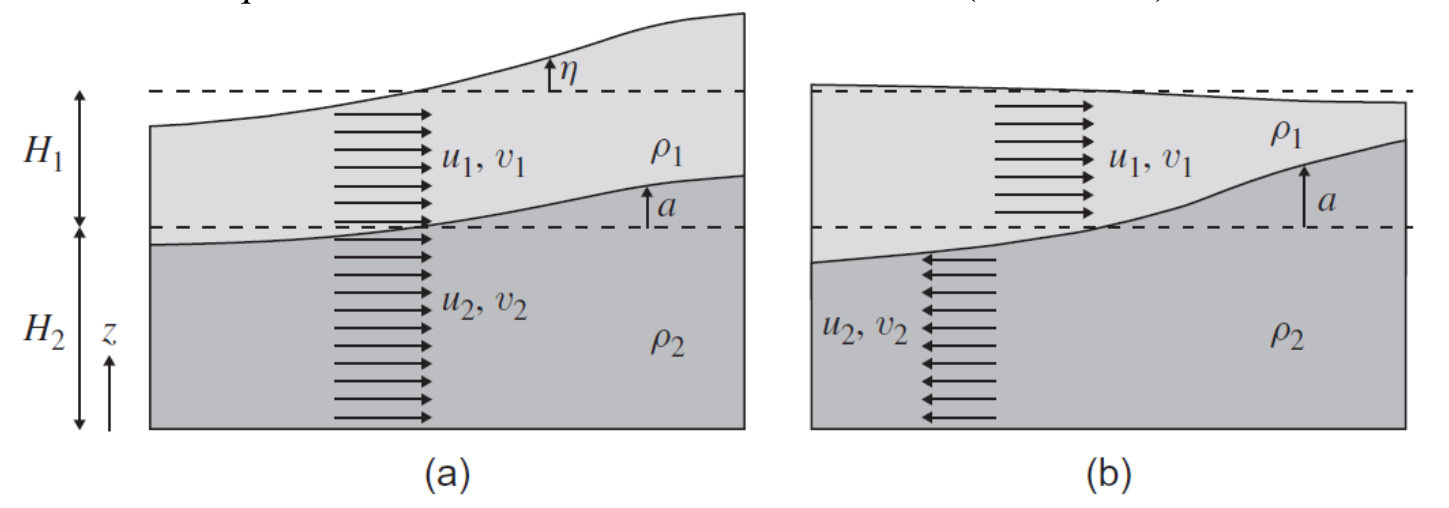
\includegraphics{/home/tparente/danilo/mestrado/github/IOF814/Lista03/outputs/modelo2camadas.png}}}
\caption{Fig 2.1 - Modelo de duas camadas.}
\label{fig2:1}
\end{figure}

    \subparagraph{Exercício 3}\label{exercuxedcio-3}

Lembrando que a equação da velocidade vertical é dada por:

\begin{equation}
    \frac{\partial{z}}{\partial{t}} = w
    \label{eq:3.1}
\end{equation}

e a equação da conservação do sal é dada por:

\begin{equation}
    \frac{\partial{S}}{\partial{t}} + \frac{\partial{uS}}{\partial{x}} + \frac{\partial{vS}}{\partial{y}} + \frac{\partial{wS}}{\partial{z}} = D_H\bigg( \frac{\partial^2{S}}{\partial{x^2}} + \frac{\partial^2{S}}{\partial{y^2}} \bigg) + D_v\frac{\partial^2{S}}{\partial{z^2}} + F_s
    \label{eq:3.2}
\end{equation}

Sabendo que a coordenada sigma se tornará a nova coordenada vertical do
sistema de coordenadas e partindo da seguinte relação para a coordenada
sigma:

\begin{equation}
    \sigma = \frac{z - \zeta}{D}, \text{ sendo: } D = H + \zeta
\end{equation}

Podemos reescrever as derivadas da seguinte forma:

\begin{equation}
    \frac{\partial{f}}{\partial{z}} = \frac{\partial{f}}{\partial{\sigma}}\frac{\partial{\sigma}}{\partial{z}} \rightarrow \frac{\partial{f}}{\partial{\sigma}}\frac{\partial(\frac{z - \zeta}{D})}{\partial{z}}
    \label{eq:3.4}
\end{equation}

Para resolver a derivada em (\ref{eq:3.4}), fazemos:

\begin{equation}
    \frac{\partial{\frac{z - \zeta}{D}}}{\partial{z}} = \frac{D\frac{\partial{(z - \zeta)}}{\partial{z}} - \frac{\partial{D}}{\partial{z}}(z - \zeta)}{D^2} = \frac{D}{D^2} = \frac{1}{D}
    \label{eq:3.5}
\end{equation}

Desta forma, aplicando (\ref{eq:3.5}) em (\ref{eq:3.4}), obtemos, enfim,
a derivada parcial em z como uma derivada parcial sigma:

\begin{equation}
    \frac{\partial{f}}{\partial{z}} = \frac{\partial{f}}{\partial{\sigma}}\frac{1}{D}
    \label{eq:3.6}
\end{equation}

Realizando procedimento semelhante, mas derivando em x e em y, obtemos:

\begin{equation}
    \frac{\partial{f}}{\partial{x}} \bigg|_z=  \frac{\partial{f}}{\partial{x}} \bigg|_\sigma + \frac{\partial{f}}{\partial{\sigma}}\frac{\partial{\sigma}}{\partial{x}} \rightarrow \frac{\partial{f}}{\partial{\sigma}}\frac{\partial(\frac{z - \zeta}{D})}{\partial{x}} \rightarrow \frac{\partial{f}}{\partial{x}} \bigg|_\sigma +\frac{1}{D}\frac{\partial{f}}{\partial{\sigma}}\bigg( \frac{\partial{\zeta}}{\partial{x}} - \sigma\frac{\partial{D}}{\partial{x}} \bigg)
    \label{eq:3.7}
\end{equation}

\begin{equation}
    \frac{\partial{f}}{\partial{y}}\bigg|_z = \frac{\partial{f}}{\partial{y}}\bigg|_\sigma + \frac{1}{D}\frac{\partial{f}}{\partial{\sigma}}\bigg( \frac{\partial{\zeta}}{\partial{y}} - \sigma\frac{\partial{D}}{\partial{y}} \bigg)
    \label{eq:3.8}
\end{equation}

E, para t, temos:

\begin{equation}
    \frac{\partial{f}}{\partial{t}}\bigg|_z = \frac{\partial{f}}{\partial{t}}\bigg|_\sigma +
    \frac{\partial{1}}{\partial{D}}\frac{\partial{f}}{\partial{\sigma}}\frac{\partial{\zeta}}{\partial{t}}(1 - \sigma)
    \label{eq:3.9}
\end{equation}

Sendo assim, aplicamos as equações obtidas acima em (\ref{eq:3.2}),
obtendo:

\begin{equation}
    \frac{\partial{S}}{\partial{t}} + \frac{1}{D}\frac{\partial{S}}{\partial{\sigma}}\frac{\partial{\zeta}}{\partial{t}}(1 - \sigma) +
    u\bigg[ \frac{\partial{S}}{\partial{x}} + \frac{Q_x}{D}\frac{\partial{S}}{\partial{\sigma}} \bigg] +
    v\bigg[ \frac{\partial{S}}{\partial{y}} + \frac{Q_y}{D}\frac{\partial{S}}{\partial{\sigma}} \bigg] +
    w\frac{1}{D}\frac{\partial{S}}{\partial{\sigma}} =
    D_H\bigg( \frac{\partial^2{S}}{\partial{x^2}} + \frac{Q_x}{D}\frac{\partial}{\partial{\sigma}}\frac{\partial{S}}{\partial{x}} +
    \frac{\partial}{\partial{x}}\frac{Q_x}{D}\frac{\partial{S}}{\partial{\sigma}} + \frac{Q^{2}_x}{D^2}\frac{\partial^2{S}}{\partial{\sigma^2}} + \frac{\partial^2{S}}{\partial{y^2}} + \frac{Q_y}{D}\frac{\partial}{\partial{\sigma}}\frac{\partial{S}}{\partial{y}} + \frac{\partial}{\partial{y}}\frac{Q_y}{D}\frac{\partial{S}}{\partial{\sigma}} + \frac{Q^{2}_y}{D^2}\frac{\partial^2{S}}{\partial{\sigma^2}} \bigg) + D_v\frac{1}{D^2}\frac{\partial^2{S}}{\partial{\sigma^2}} + F_S
    \label{eq:3.10}
\end{equation}

Sendo que:

\begin{equation}
    Q_x = \frac{\partial{\zeta}}{\partial{x}} - \sigma \frac{\partial{D}}{\partial{x}} \\
    Q_y = \frac{\partial{\zeta}}{\partial{y}} - \sigma \frac{\partial{D}}{\partial{y}} \\
\end{equation}

E, para a velocidade vertical, consideramos que:

\begin{equation}
    z = D\sigma + \zeta
\end{equation}

Então,

\begin{equation}
    w = \frac{dz}{dt} \rightarrow \frac{d(D\sigma + \zeta)}{dt} \rightarrow
    \frac{\partial{[(H + \zeta)\sigma + \zeta]}}{\partial{t}} + u\bigg[ \frac{\partial{[(H + \zeta)\sigma + \zeta]}}{\partial{x}} + v\bigg[ \frac{\partial{[(H + \zeta)\sigma + \zeta]}}{\partial{y}} \bigg] \rightarrow  \\
    D\frac{\partial{\sigma}}{\partial{t}} + \sigma\frac{\partial{\zeta}}{\partial{t}} + \frac{\partial{\zeta}}{\partial{t}} + u\bigg[ D\frac{\partial{\sigma}}{\partial{x}} + \sigma\frac{\partial{D}}{\partial{x}} + \frac{\partial{\zeta}}{\partial{x}} \bigg] + v\bigg[ D\frac{\partial{\sigma}}{\partial{y}} + \sigma\frac{\partial{D}}{\partial{y}} + \frac{\partial{\zeta}}{\partial{y}} \bigg] \rightarrow \\
    D\frac{\partial{\sigma}}{\partial{t}} + (\sigma + 1)\frac{\partial{\zeta}}{\partial{t}} + u\bigg[ \sigma\frac{\partial{D}}{\partial{x}} + \frac{\partial{\zeta}}{\partial{x}} \bigg] + \frac{\partial}{\partial{\sigma}}v\bigg( \sigma\frac{\partial{D}}{\partial{y}} + \frac{\partial{\zeta}}{\partial{y}} \bigg)
    \label{eq:3.11}
\end{equation}

Portando, teremos:

\begin{equation}
    \frac{\partial{w}}{\partial{\sigma}} = \frac{\partial}{\partial{\sigma}}\bigg[ D\frac{\partial{\sigma}}{\partial{t}} + (\sigma + 1)\frac{\partial{\zeta}}{\partial{t}} \bigg] + \frac{\partial}{\partial{\sigma}}\bigg[ u\bigg( \sigma\frac{\partial{D}}{\partial{x}} + \frac{\partial{\zeta}}{\partial{x}} \bigg) \bigg]+ v\bigg[ \sigma\frac{\partial{D}}{\partial{y}} + \frac{\partial{\zeta}}{\partial{y}} \bigg]
\end{equation}

    \subparagraph{Exercício 04}\label{exercuxedcio-04}

Partindo de um sistema de equações hidrodinâmicas básicas em 3 dimensões
e simplificada (sem termos advectivos e sem difusão horizontal):

\begin{equation}
    \frac{\partial{\eta}}{\partial{t}} + \frac{\partial}{\partial{x}}\int_{0}^{D}udz + \frac{\partial}{\partial{y}}\int_{0}^{D}vdz = 0
    \\
    \frac{\partial{u}}{\partial{t}} - fv = -g\frac{\partial{\eta}}{\partial{x}} - \frac{1}{\rho}\frac{\partial{p_a}}{\partial{x}} + \frac{\partial}{\partial{z}}\bigg( N\frac{\partial{u}}{\partial{z}} \bigg)
    \\
    \frac{\partial{v}}{\partial{t}} + fu = -g\frac{\partial{\eta}}{\partial{y}} - \frac{1}{\rho}\frac{\partial{p_a}}{\partial{y}} + \frac{\partial}{\partial{z}}\bigg( N\frac{\partial{v}}{\partial{z}} \bigg)
    \label{eq:4.1}
\end{equation}

Com as seguintes condições de contorno na superfície:

\begin{equation}
    \tau_{xs} = -\rho\bigg( N\frac{\partial{u}}{\partial{z}} \bigg)
    \\
    \tau_{ys} = -\rho\bigg( N\frac{\partial{v}}{\partial{z}} \bigg)
    \label{eq:4.2}
\end{equation}

E, no fundo:

\begin{equation}
    \tau_{xB} = K_b\rho u_D
    \\
    \tau_{yB} = K_b\rho v_ D
    \label{eq:4.3}
\end{equation}

Igualando (\ref{eq:4.2}) e (\ref{eq:4.3}), obtemos:

\begin{equation}
    \bigg( N\frac{\partial{u}}{\partial{z}} \bigg)_D + K_b u_D = 0
    \\
    \bigg( N\frac{\partial{v}}{\partial{z}} \bigg)_D + K_b v_ D = 0
    \label{eq:4.4}
\end{equation}

Definimos, assim, as transformadas das componentes de corrente (u e v)
através das auto-funções \(f_r\), associadas aos auto-valores
\(\lambda_r\):

\begin{equation}
    u_r = \frac{1}{D}\int^{D}_{0}u f_r(z) dz
    \\
    v_r = \frac{1}{D}\int^{D}_{0}v f_r(z) dz
    \label{eq:4.5}
\end{equation}

Aplicando o operador de transformada (\ref{eq:4.5}) nos termos de
(\ref{eq:4.1}), obtemos:

\begin{equation}
    \frac{\partial{u_r}}{\partial{t}} - fv_r = -ga_r\frac{\partial{\eta}}{\partial{x}} - \frac{1}{\rho}a_r\frac{\partial{p_a}}{\partial{x}} + \frac{1}{D}\int^{D}_{0}f_r(z)\frac{\partial}{\partial{z}}\bigg( N\frac{\partial{u}}{\partial{z}} \bigg)dz
    \\
    \frac{\partial{v_r}}{\partial{t}} + fu_r = -ga_r\frac{\partial{\eta}}{\partial{y}} - \frac{1}{\rho}a_r\frac{\partial{p_a}}{\partial{y}} + \frac{1}{D}\int^{D}_{0}f_r(z)\frac{\partial}{\partial{z}}\bigg( N\frac{\partial{v}}{\partial{z}} \bigg)dz
    \label{eq:4.6}
\end{equation}

onde:

\begin{equation}
    a_r = \frac{1}{D}\int^{D}_{0}f_r(z)dz
    \label{eq:4.7}
\end{equation}

Podemos determinar as auto-funções \(f_r\) e os auto-valores
\(\lambda_r\) utilizando a representação da difusão como decaimento,
sendo que o efeito será máximo na superfície e (\ref{eq:4.4}) no fundo
será:

\begin{equation}
    \frac{d}{dz}\bigg[ Nf'_r(z) \bigg] = -\lambda_r f_r(z)
\end{equation}

\begin{equation}
    f_r(0) = 1
    \label{eq:4.8}
\end{equation}

\begin{equation}
    f'_r(0) = 0
    \label{eq:4.9}
\end{equation}

\begin{equation}
    N f'_r(D) + K f_r(D) = 0
    \label{eq:4.10}
\end{equation}

Desta forma, reescrevemos (\ref{eq:4.6}) como:

\begin{equation}
    \frac{\partial{u_r}}{\partial{t}} - fv_r = -ga_r\frac{\partial{\eta}}{\partial{x}} - \frac{1}{\rho}a_r\frac{\partial{p_a}}{\partial{x}} + \frac{\tau_{xs}}{\rho D} - \lambda_ru_r
    \\
    \frac{\partial{v_r}}{\partial{t}} + fu_r = -ga_r\frac{\partial{\eta}}{\partial{y}} - \frac{1}{\rho}a_r\frac{\partial{p_a}}{\partial{y}} + \frac{\tau_{ys}}{\rho D} - \lambda_rv_r
    \label{eq:4.11}
\end{equation}

Sendo que a determinação das componentes u e v são feitos através de
expansões do tipo:

\begin{equation}
    u = \sum^{\infty}_{r=l} A_rf_r(z)
    \\
    v = \sum^{\infty}_{r=l} B_rf_r(z)
    \label{eq:4.12}
\end{equation}

Da condição de ortogonalidade das auto-funções, podemos calcular os
coeficientes das expansões:

\begin{equation}
    \int^{D}_{0}f_r(z) f_s(z) dz = 0, r \neq s
    \\
    \int^{D}_{0}f^{2}_{r}(z) dz = I_r(D) - I_r(0)
    \\
    \text{onde, } I_r(z) = N\bigg[ f'\frac{\partial{f}}{\partial{\lambda}} - f\frac{\partial{f'}}{\partial{\lambda}} \bigg]_{\lambda=\lambda_r}
    \label{eq:4.13}
\end{equation}

Por fim,

\begin{equation}
    u = \sum^{\infty}_{r=l} \phi_r u_r f_r(z)
    \\
    v = \sum^{\infty}_{r=l} \phi_r v_r f_r(z)
    \label{eq:4.14}
\end{equation}

\begin{equation}
    \phi_r = \frac{D}{I_r(D) - I_r(0)}
    \label{eq:4.15}
\end{equation}

Com as transformadas das correntes, podemos escrever a equação da
continuidade como:

\begin{equation}
    \frac{\partial{\eta}}{\partial{t}} + \sum^{\infty}_{r=l}\bigg( \frac{\partial}{\partial{x}}(D a_r \phi_r u_r) + \frac{\partial}{\partial{y}}D a_r \phi_r v_r \bigg) = 0
\end{equation}

E, finalmente, obtemos a componente vertical da velocidade:

\begin{equation}
    w + \sum^{\infty}_{r=l}\bigg( \frac{\partial}{\partial{x}}(\phi_r u_r\int^{D}_{z}f_r(z)dz) + \frac{\partial}{\partial{y}}(\phi_r v_r\int^{D}_{z}f_r(z)dz) \bigg) = 0
\end{equation}

Portanto, as equações do modelo são substituídas pelas equações
transformadas para \(\eta\), u e v obtidas no desenvolvimento do
exercício.

    \subparagraph{Exercício 5}\label{exercuxedcio-5}

Modelou-se a região de Santos para ventos variando a cada 3 horas,
simulando uma condição de evento metereológico de passagem de sistemas
frontais, com ventos do quadrante Sul com intensidade de
\(10 m.s^{-1}\). Além disso, considerou-se uma elevação senoidal nos
contornos abertos, simulando a maré. Desta forma, os resultados obtidos,
embora inadequados para análises dentro da Baía de Santos, são
apresentados abaixo.

O campo batimétrico (Fig 5.1) utilizado foi extraído do etopo1, onde
utilizou-se os valores maiores que zero como região de continente,
gerando-se as chaves 0 (para terra) e 1 (para mar), conforme Fig 5.2.


\begin{figure}[!ht]
\centering
\centerline{\hbox{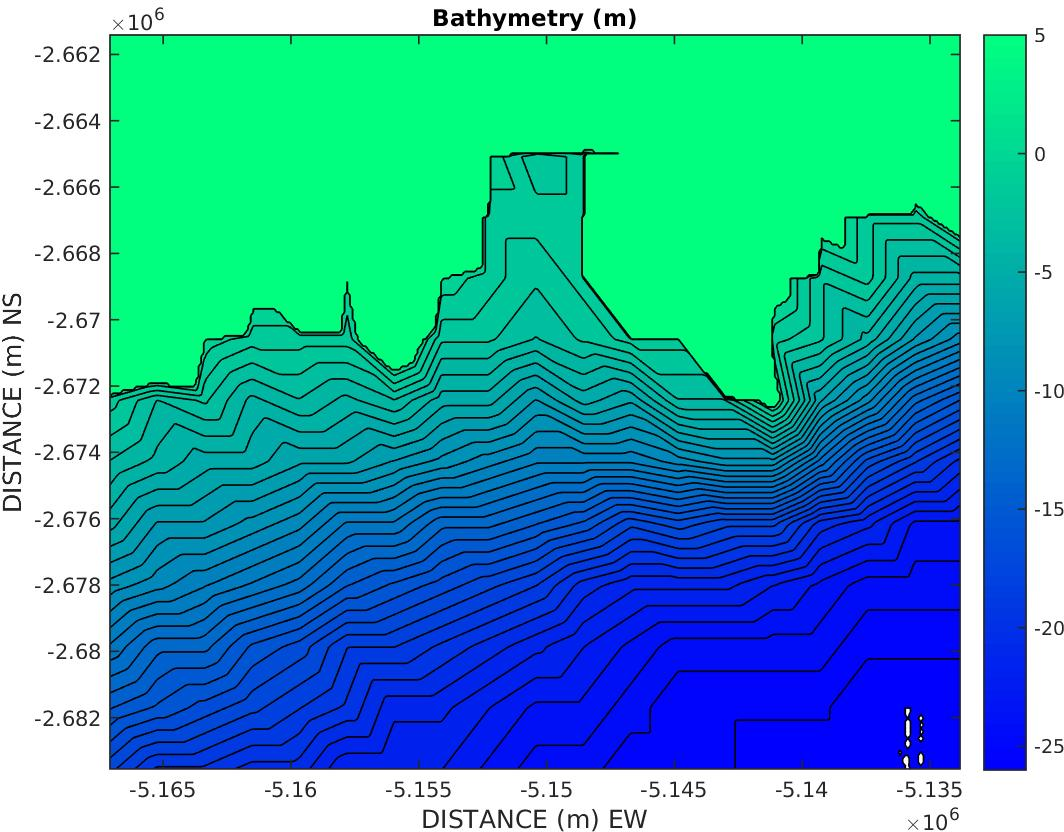
\includegraphics{/home/tparente/danilo/mestrado/github/IOF814/Lista03/outputs/ex05/bathymetry.png}}}
\caption{Fig 5.1 - Campo batimétrico extraído do ETOPO1.}
\label{fig5:1}
\end{figure}

\begin{figure}[!ht]
\centering
\centerline{\hbox{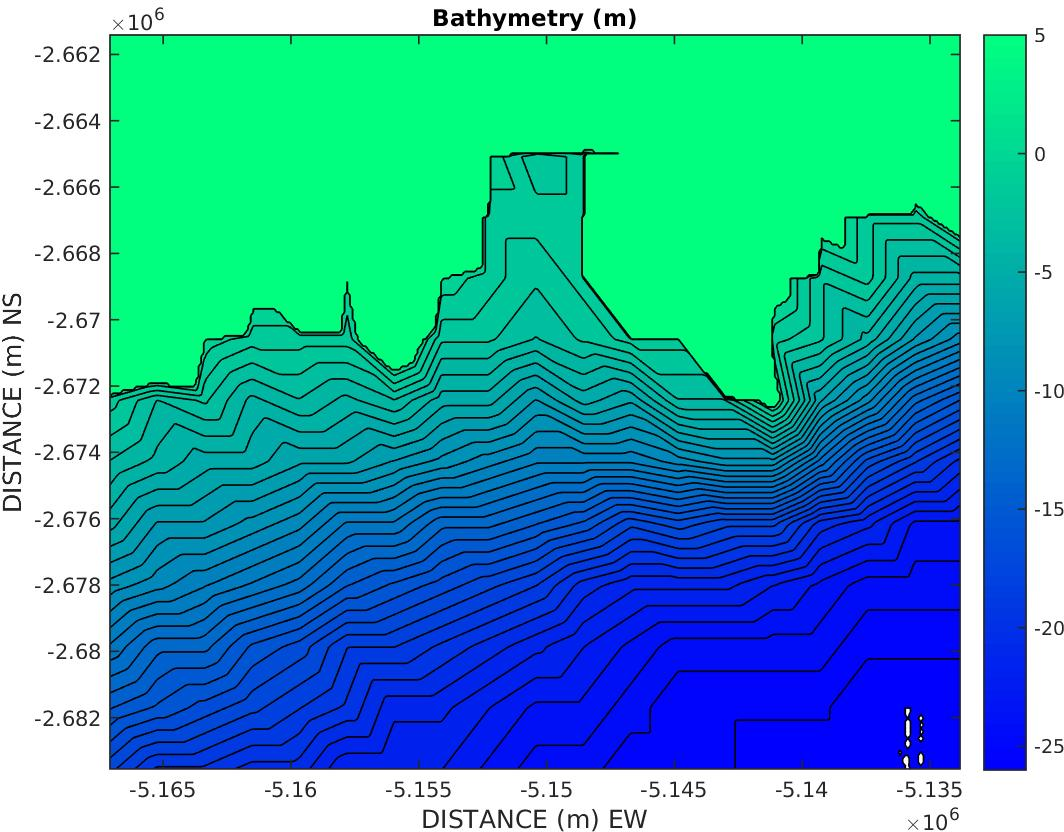
\includegraphics{/home/tparente/danilo/mestrado/github/IOF814/Lista03/outputs/ex05/bathymetry.png}}}
\caption{Fig 5.2 - Chaves utilizada para realizar cálculos somente nas células oceânicas.}
\label{fig5:2}
\end{figure}

Os campos de corrente e elevação da superfície livre do mar foram
plotados sempre um instante anterior à mudança do vento, representando
um instante de estabilidade do modelo, com o equilíbrio atingido. Foi
analisado os campos de correntes em três profundidades: superfície, 5m e
10m.

\begin{figure}[!ht]
\centering
\centerline{\hbox{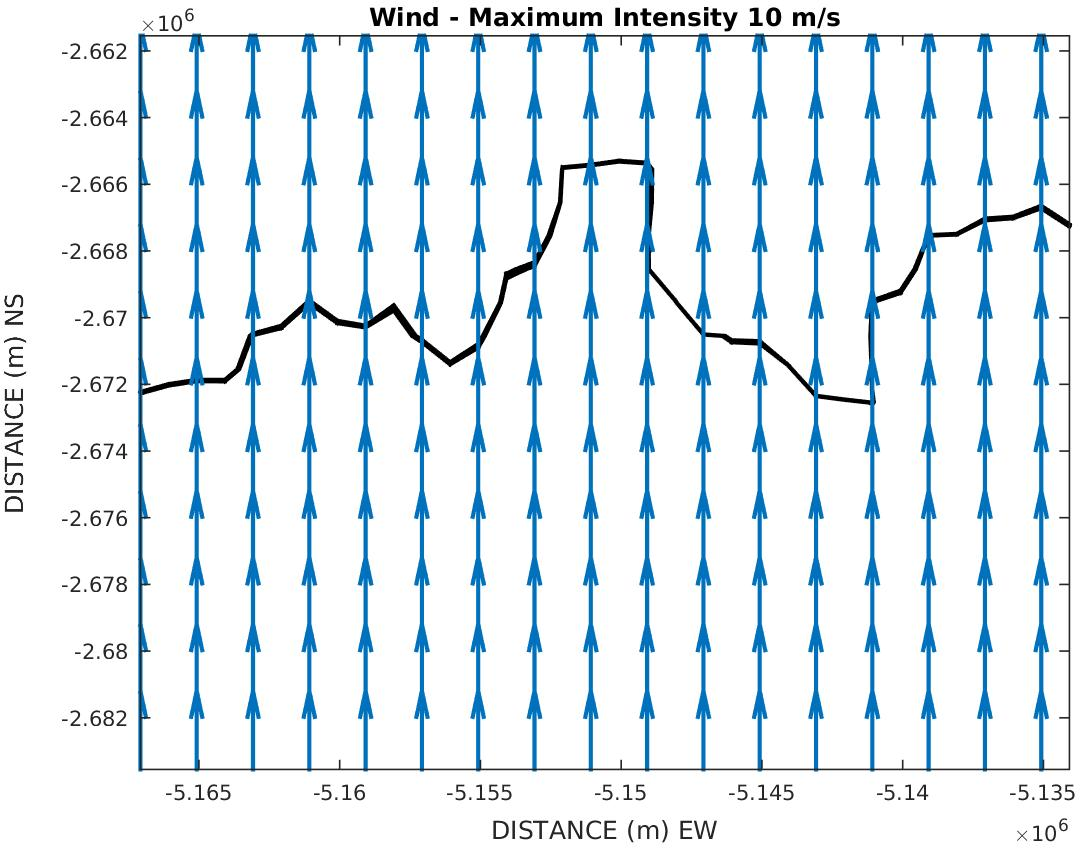
\includegraphics{/home/tparente/danilo/mestrado/github/IOF814/Lista03/outputs/ex05/windField_S.png}}}
\caption{Fig 5.3 - Campo de ventos de sul utilizados nas primeiras horas de simulação.}
\label{fig5:3}
\end{figure}

\begin{figure}[!ht]
\centering
\centerline{\hbox{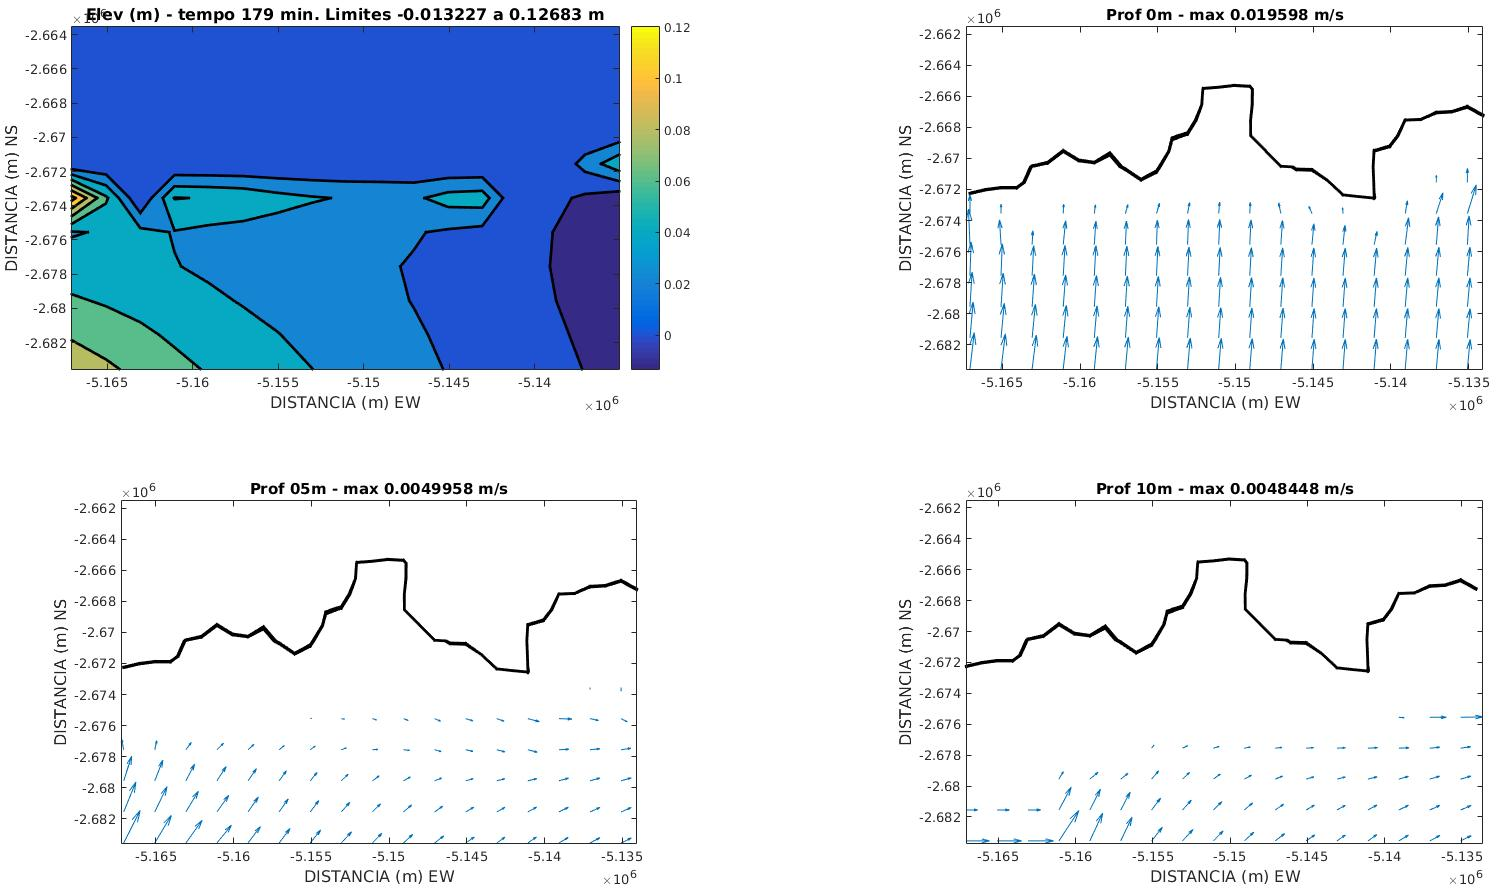
\includegraphics{/home/tparente/danilo/mestrado/github/IOF814/Lista03/outputs/ex05/ventodeSul.png}}}
\caption{Fig 5.4 - Resposta do nível do mar (superior esquerdo) e do campo de correntes na superfície (superior direito), a 5 metros de profundidade (inferior esquerdo) e
10 metros de profundidade (inferior direito).}
\label{fig5:4}
\end{figure}

\begin{figure}[!ht]
\centering
\centerline{\hbox{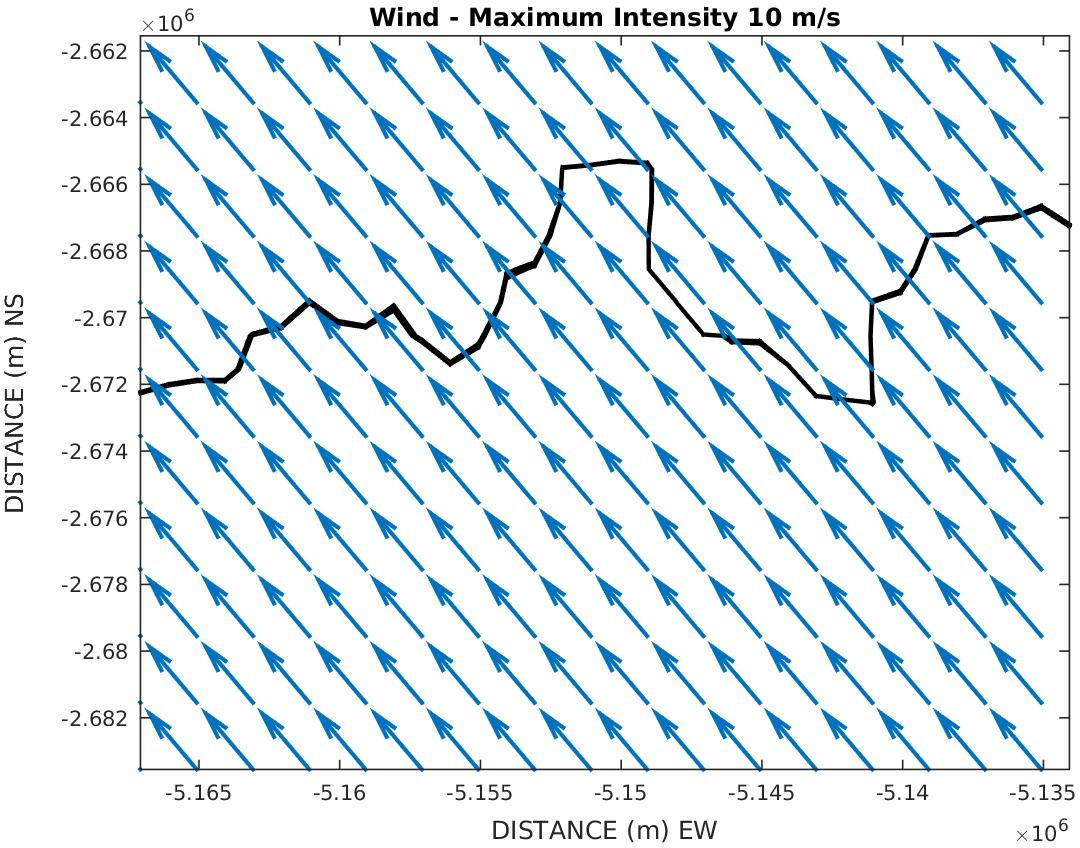
\includegraphics{/home/tparente/danilo/mestrado/github/IOF814/Lista03/outputs/ex05/windField_SE.png}}}
\caption{Fig 5.5 - Campo de ventos de sudeste utilizados entre 3 e 6 horas de simulação.}
\label{fig5:5}
\end{figure}

\begin{figure}[!ht]
\centering
\centerline{\hbox{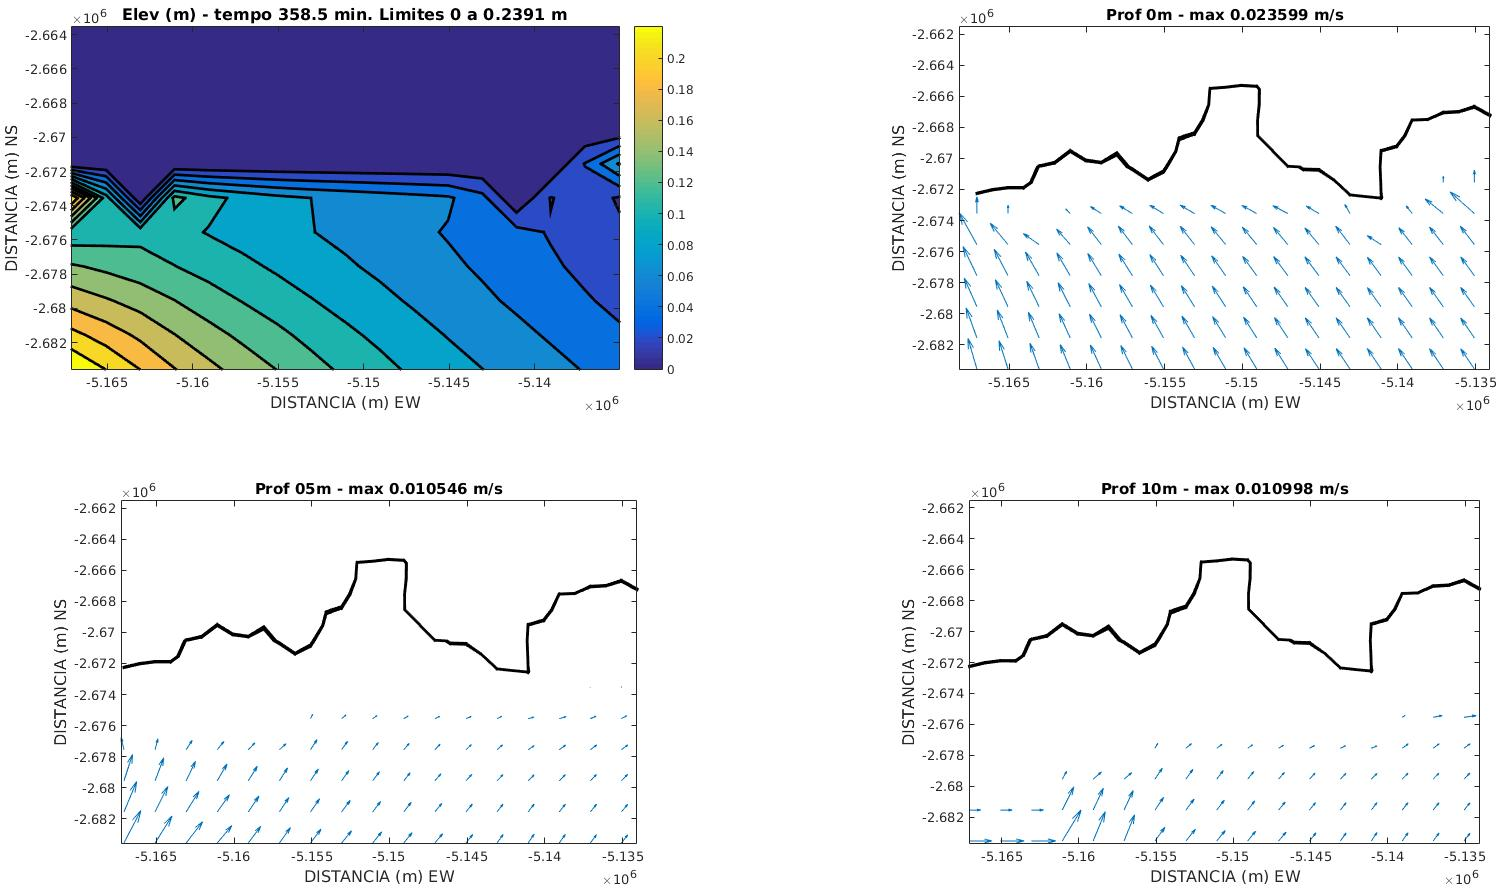
\includegraphics{/home/tparente/danilo/mestrado/github/IOF814/Lista03/outputs/ex05/ventodeSE.png}}}
\caption{Fig 5.6 - Idem Fig 5.4}
\label{fig5:6}
\end{figure}

\begin{figure}[!ht]
\centering
\centerline{\hbox{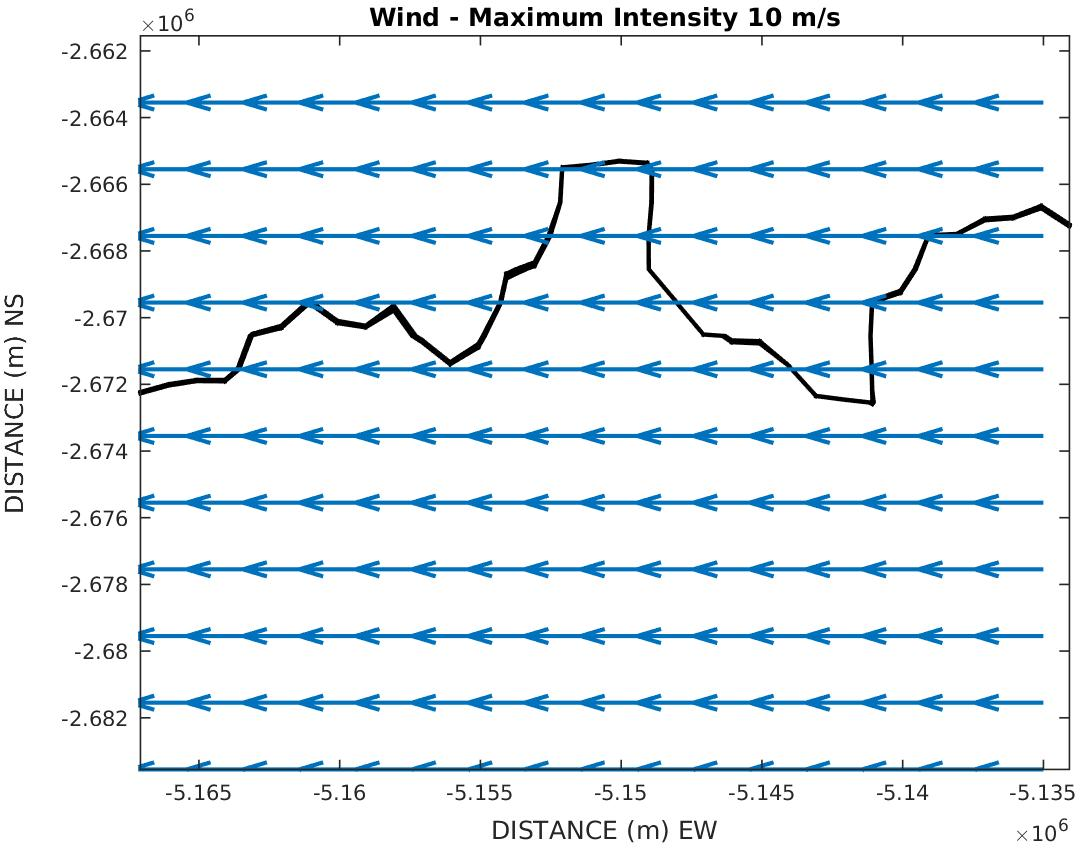
\includegraphics{/home/tparente/danilo/mestrado/github/IOF814/Lista03/outputs/ex05/windField_E.png}}}
\caption{Fig 5.7 - Campo de ventos de leste utilizados entre 6 e 9 horas de simulação.}
\label{fig5:7}
\end{figure}

\begin{figure}[!ht]
\centering
\centerline{\hbox{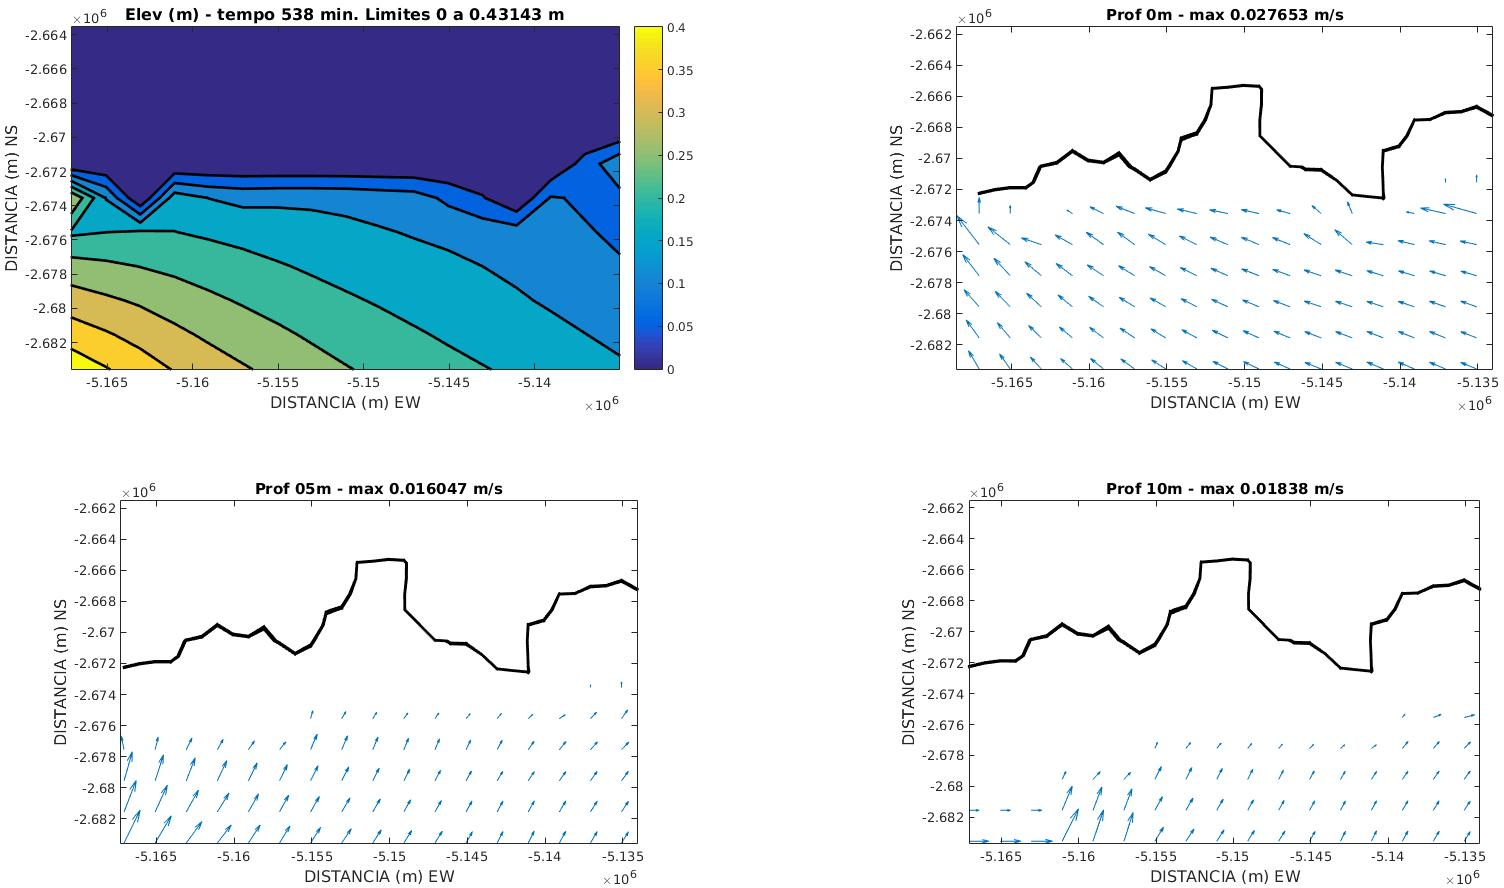
\includegraphics{/home/tparente/danilo/mestrado/github/IOF814/Lista03/outputs/ex05/ventodeE.png}}}
\caption{Fig 5.8 - Idem Fig 5.4}
\label{fig5:8}
\end{figure}

\begin{figure}[!ht]
\centering
\centerline{\hbox{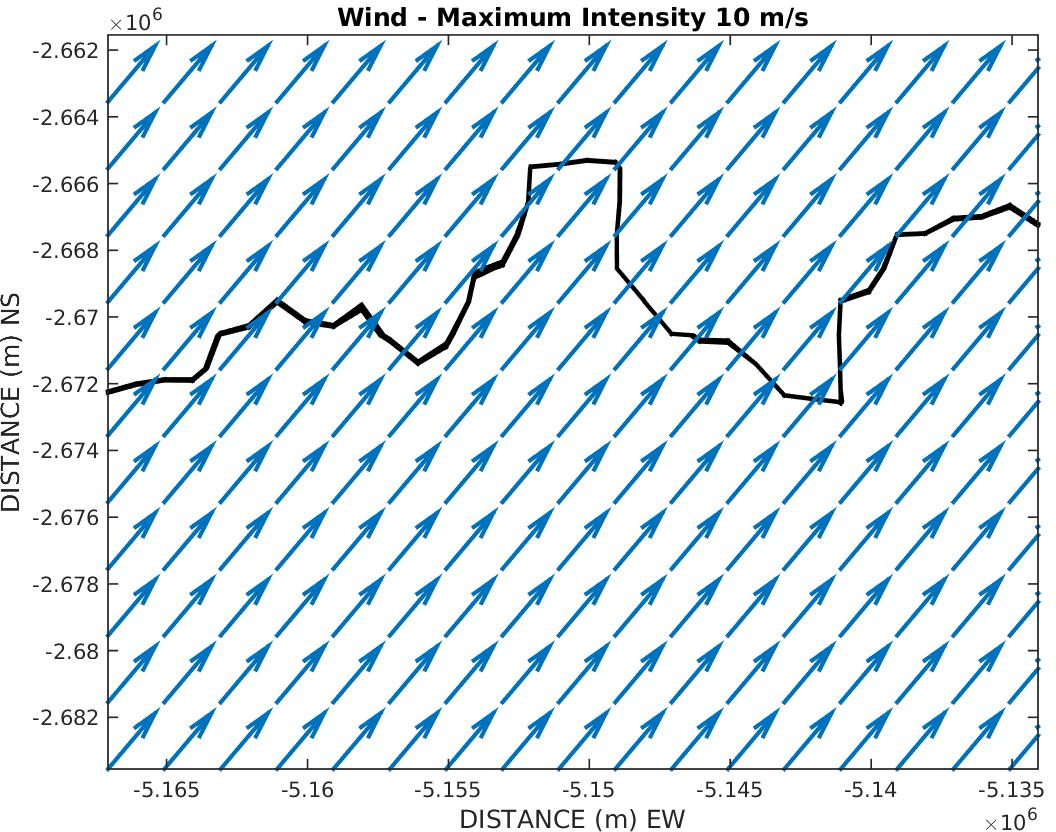
\includegraphics{/home/tparente/danilo/mestrado/github/IOF814/Lista03/outputs/ex05/windField_SW.png}}}
\caption{Fig 5.9 - Campo de ventos de sudeste utilizados nas 3 horas finais de simulação.}
\label{fig5:9}
\end{figure}

\begin{figure}[!ht]
\centering
\centerline{\hbox{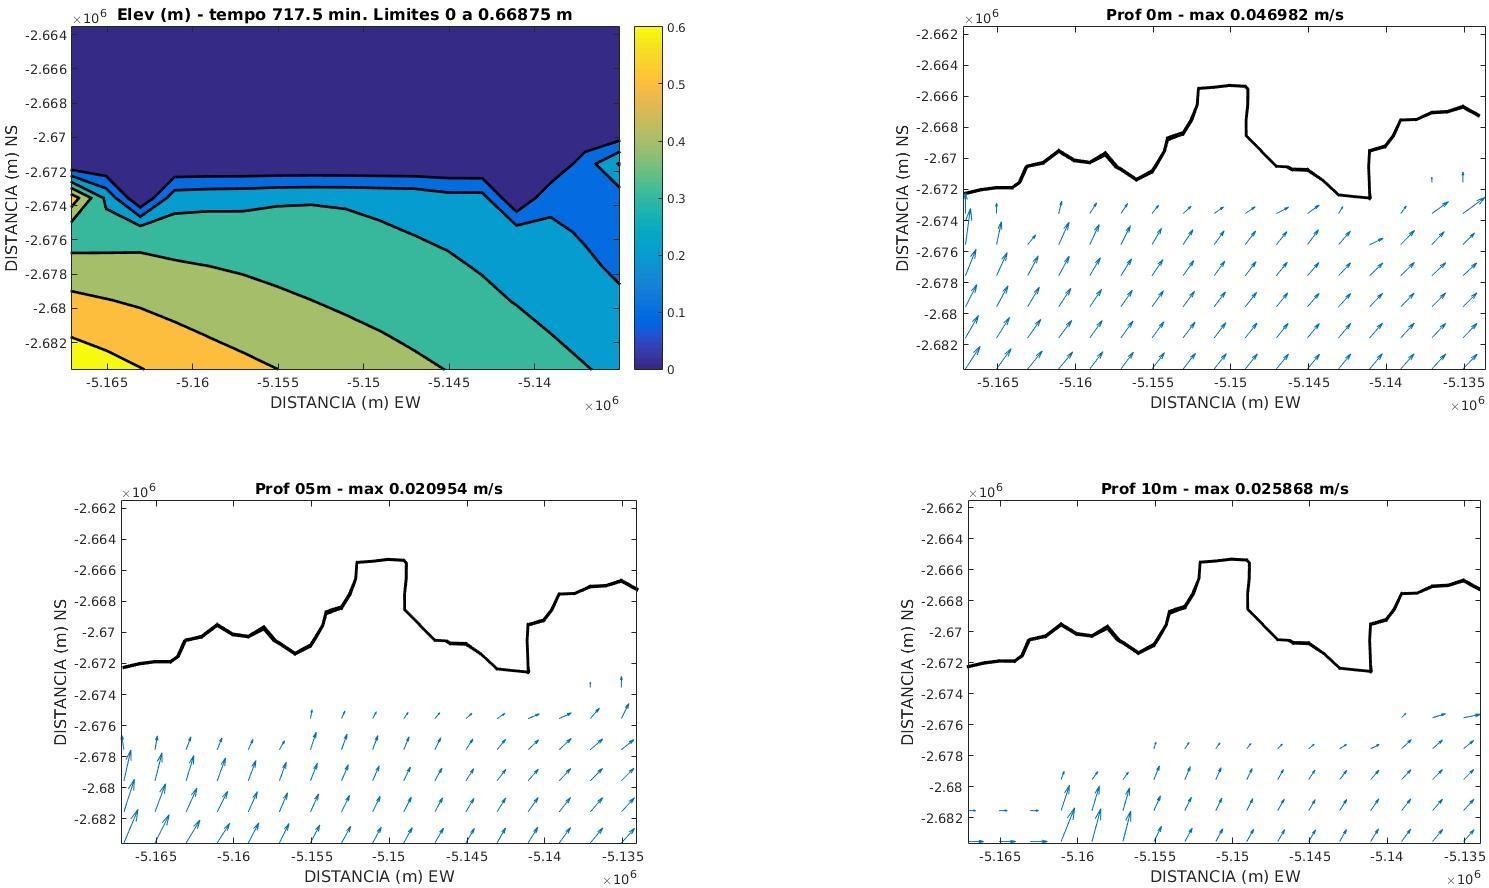
\includegraphics{/home/tparente/danilo/mestrado/github/IOF814/Lista03/outputs/ex05/ventodeSW.png}}}
\caption{Fig 5.10 - Idem Fig 5.4}
\label{fig5:10}
\end{figure}

Por algum motivo não identificado pelo aluno, o modelo não processou
regiões mais costeiras, obtendo resultados somente na porção offshore do
domínio modelado.

Por fim, as séries temporais em dois pontos de interesse foram analisadas (Fig 5.11 e 5.12), onde no ponto
mais interno, dentro da Baía de Santos, não foram observadas correntes devido ao problema já discutido acima.
Obtivemos então, somente uma série temporal válida para o ponto de interesse mais offshore, próximo ao contorno
aberto do domínio modelado.

\begin{figure}[!ht]
\centering
\centerline{\hbox{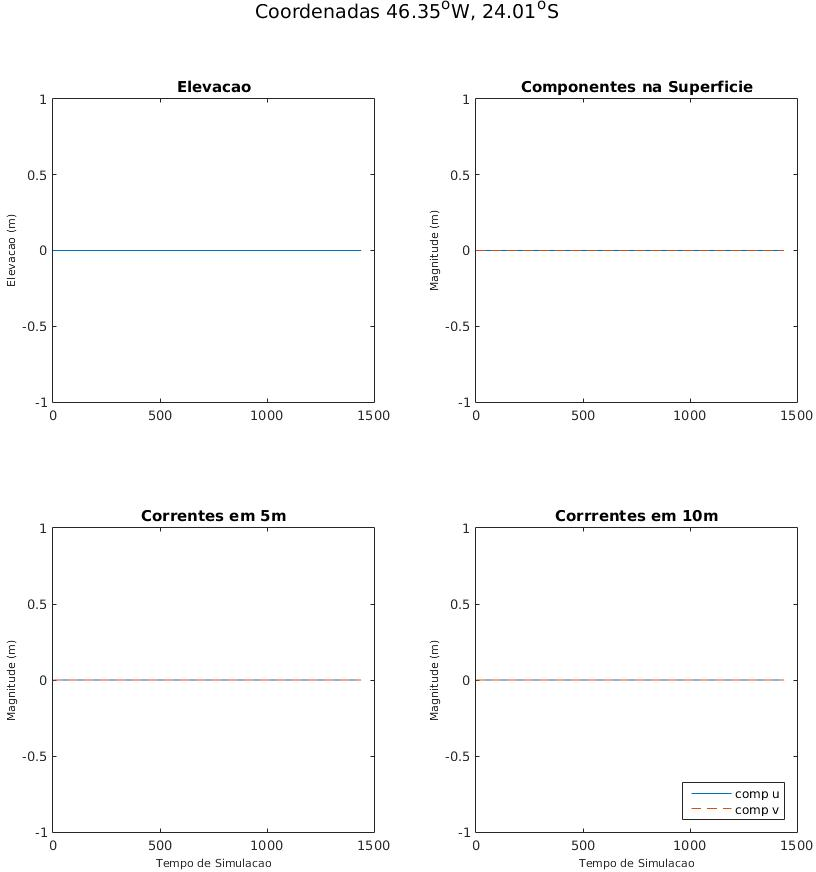
\includegraphics{/home/tparente/danilo/mestrado/github/IOF814/Lista03/outputs/ex05/santos.png}}}
\caption{Fig 5.11 - Série temporal para região de interesse dentro da Baía de Santos, para os mesmos parâmetros apresentados na Fig 5.4.}
\label{fig5:9}
\end{figure}

\begin{figure}[!ht]
\centering
\centerline{\hbox{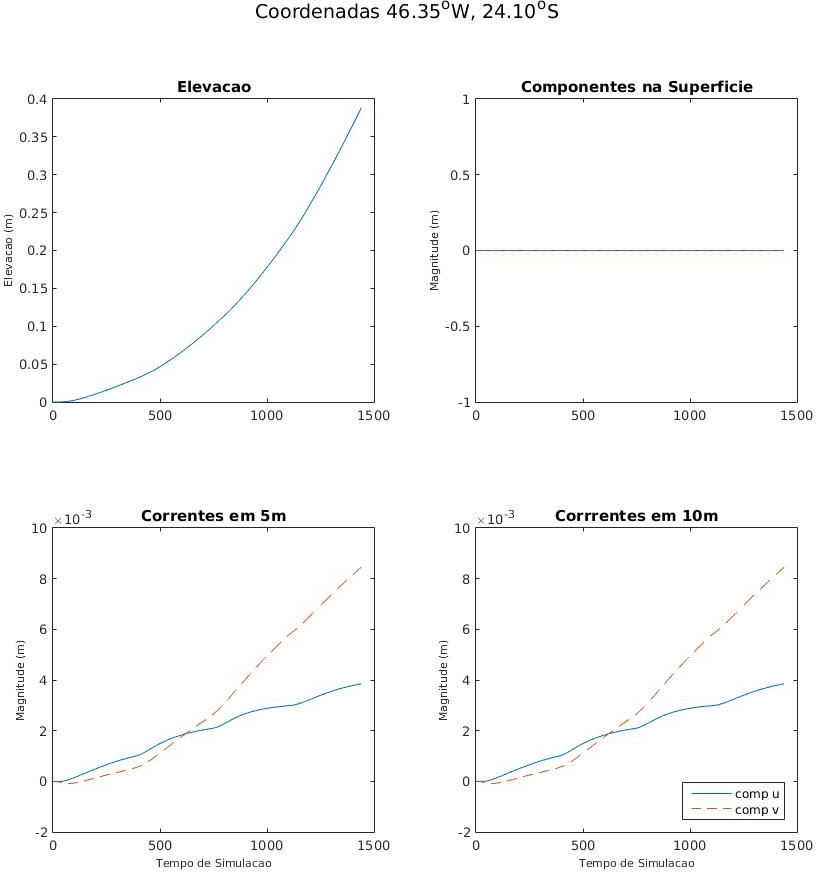
\includegraphics{/home/tparente/danilo/mestrado/github/IOF814/Lista03/outputs/ex05/offshore.png}}}
\caption{Fig 5.12 - Idem Fig 5.11, mas para ponto de interesse offshore.}
\label{fig5:12}
\end{figure}

    % Add a bibliography block to the postdoc



    \end{document}
